\documentclass[10pt, a4j, dvipdfmx]{jarticle}
\usepackage{titlesec}
\usepackage[dvipdfmx]{graphicx}
\usepackage{float}
\usepackage{wrapfig}
\usepackage{subfigure}
\usepackage{caption}

\makeatletter
\newcommand{\figcaption}[1]{\def\@captype{figure}\caption{#1}}
\newcommand{\tblcaption}[1]{\def\@captype{table}\caption{#1}}
\makeatother

\title{ディジタル回路I}
\author{4年 電子システム工学科 40番  山地 駿徹}

\begin{document}
%\maketitle

\section{目的}
この実験課題はディジタル回路の基礎的特性測定を通し,ディジタルICの特性に関する基礎概念並びに測定技術の習得を目的をする.

\section{原理}
集積回路 (IC = Integrated Circuit) のIntegrated(集積)の意味は,1つの基盤にお互いに分離できない状態で回路素子が結合されているということで,半導体集積回路(monolithic)と薄膜集積回路(thin film)および両者を併用した混成集積回路(hybrid)とがある.
半導体集積回路にはバイポーラトランジスタを用いたものとMOSトランジスタを用いたものがあり,後者のほうが高集積密度のものを作りやすい.
ディジタルICにはDTL,TTL,ECL,CMOS等種々の回路形式がありそれぞれ特徴がある.

\subsection*{電圧反転機(inverter)}
集積回路について述べる前にCMOS反転機について簡単に説明する.
nチャンネルMOSFETとpチャンネルMOSFETを相補的に接続したCMOSの反転(インバータ)回路を図1に示す.
入力電圧$V_i$ が低レベルの電圧(L)のときは,$T_p$のゲート・ソース間は0Vになるためオフ(遮断)状態となる.
よって,出力$V_0$は高レベル(H)となる.
一方,入力電圧$V_i$が高レベルの電圧(H)のときは,$T_p$のゲート・ソース 間は0Vとなるためオフ状態となり,$T_n$のゲート・ソース間は負のバイアスが印加されるためオン状態となる.
よって出力$V_0$は低レベル(L)となる.従って,入出力特性は図2のようになる.
\begin{figure}[H]
  \begin{minipage}{0.5\hsize}
    \centering
    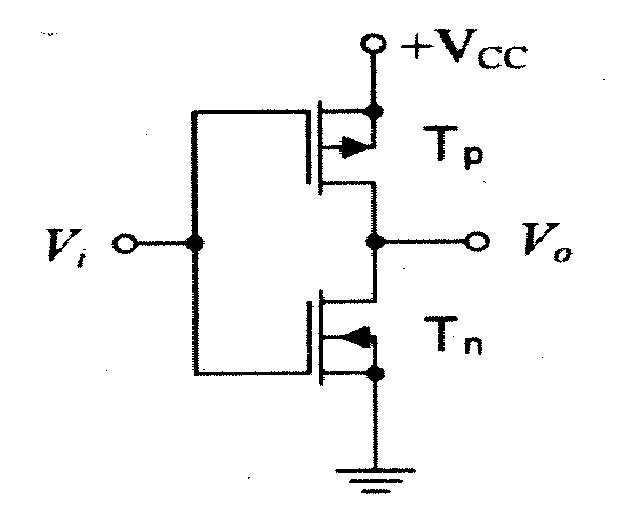
\includegraphics[height=40mm]{実験テキスト/図1.png}
    \caption{CMOS反転器}
  \end{minipage}
  \begin{minipage}{0.5\hsize}
    \centering
    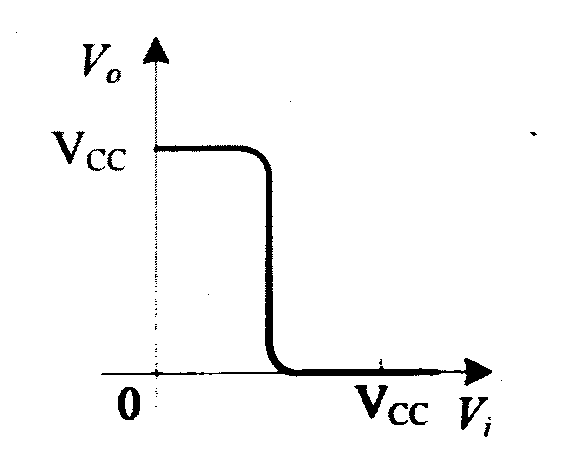
\includegraphics[height=40mm]{実験テキスト/図2.png}
    \caption{CMOS反転器の入出力特性}
  \end{minipage}
\end{figure}

\subsection*{標準CMOSの測定}
一口に集積回路といっても種々の論理特性を持ったものがあるが,ここでは代表的なCMOS IC 74HC00(NANDゲート)について考える.

74HC00の回路図を図3に示す.
この素子4組を1個としてDual-in-line packageされて製品化されている.
代表的な端子接続図を図4に示す.
図4中のNANDは図3の回路を意味する記号である.
端子14には電源電圧+5Vを印加し,端子7は共通接地点である.
以下,端子14-7間には定格電源電圧が加えられているものとする.
\begin{figure}[H]
  \begin{minipage}{0.5\hsize}
    \centering
    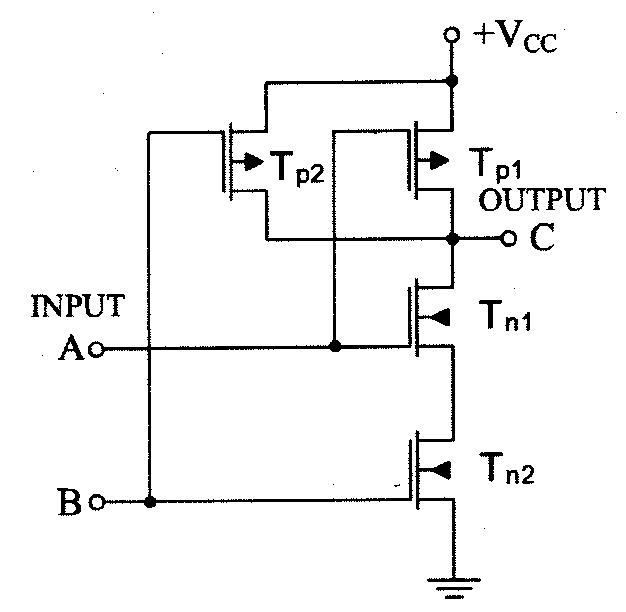
\includegraphics[height=50mm]{実験テキスト/図3.png}
    \caption{IC 74HC00の回路}
  \end{minipage}
  \begin{minipage}{0.5\hsize}
    \centering
    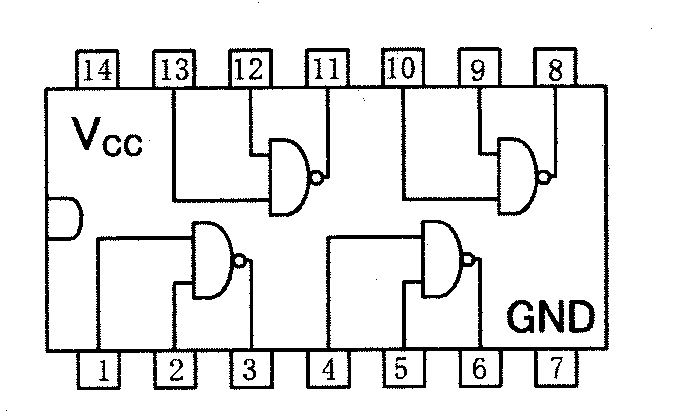
\includegraphics[height=30mm]{実験テキスト/図4.png}
    \caption{IC 74HC00の端子接続図}
  \end{minipage}
\end{figure}

図3のNANDゲートにおいて,入力A=LかつB=Lのとき,$T_{p1}$と$T_{p2}$がオン状態,$T_{n1}$と$T_{n2}$がオフ状態であるので,電源から出力に至る経路は導通状態であり出力C=Hとなる.
入力A=HかつB=L のとき,$T_{p1}$はオフ状態そして$T_{p2}$はオン状態,$T_{n1}$はオン状態そして$T_{n2}$がオフ状態であるので,出力は$T_{p2}$を通して電源と導通状態であり出力C=Hとなる.
入力A=LかつB=Hも同様に考えられ,出力C=Hとなる.
これに対して,入力A=HかつB=Hのとき,$T_{p1}$と$T_{p2}$がオフ状態,$T_{n1}$と$T_{n2}$がオン状態であるので,接地から出力に至る経路は導通状態であり出力C=Lとなる.
以上のことから,この論理ゲートがNAND機能を実装していることは明らかである.

次に,入力Bを5V一定とし,入力Aの電圧を0Vから徐々に上昇させていくことを考える.
ここで,出力Cを流れる電流は0とする.
前述のようにA電圧が低いとき$T_{p1}$はオン状態そして$T_{p2}$はオフ状態,$T_{n1}$はオフ状態そして$T_{n2}$はオン状態となっており,電源から流れ出す電流は0である.
しかし,A電圧が大きくなり出力が反転する電圧付近に近づくと$T_{n1}$はオフ状態からソース・ドレイン間に電流が流れる状態(能動状態)に変わり,$T_{p1}$と$T_{n1}$はともに能動状態となる.
このとき電源から接地に向けて電源電流が流れ,この電流を貫通電流と呼んでいる.
更に,入力Aを上昇させると$T_{p1}$はオフ状態,$T_{n1}$はオン状態となり,電源電流は流れなくなる.

\newpage
\section{実験方法}
\subsection{電源電流特性(貫通電流特性)の測定}
電源電流特性(貫通電流特性)の測定回路図を図5に,測定結果例を図6に示す.
まず,図7に示す回路を基板上に制作し,NANDの入力の片方を"1"(Highレベル=5V)に接続し,もう一方の入力には保護抵抗を介して可変電源を接続する.
\begin{figure}[H]
  \begin{minipage}{0.5\hsize}
    \centering
    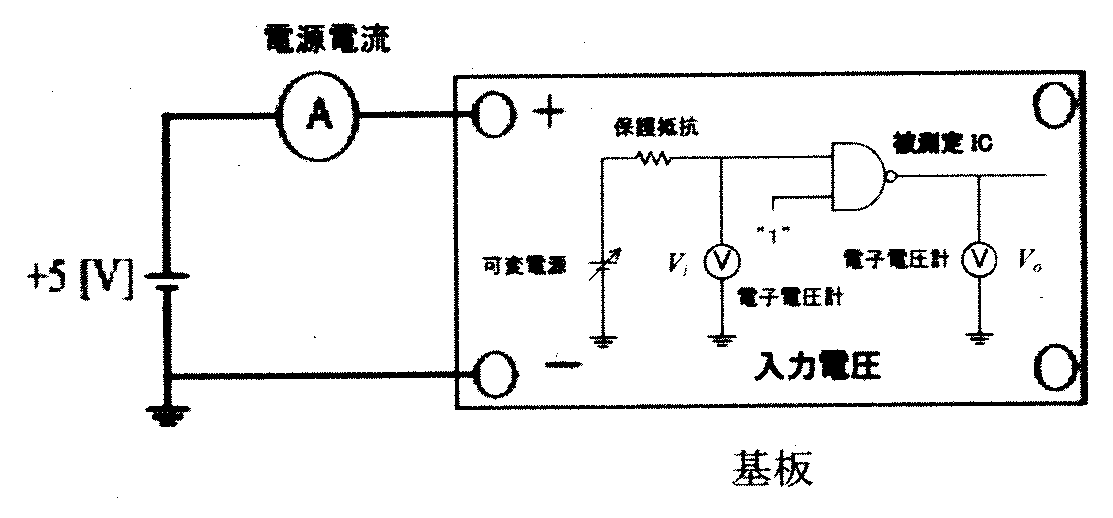
\includegraphics[width=75mm]{実験テキスト/図5.png}
    \caption{IC 74HC00の回路}
  \end{minipage}
  \begin{minipage}{0.5\hsize}
    \centering
    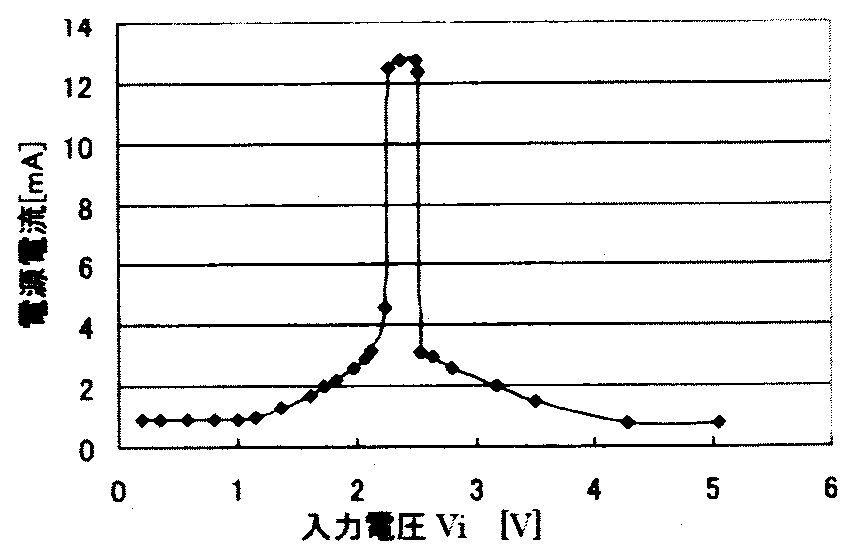
\includegraphics[height=40mm]{実験テキスト/図6.png}
    \caption{IC 74HC00の端子接続図}
  \end{minipage}
\end{figure}
可変電源の出力電圧を0Vから徐々に上げ,NANDの入力に印加する.
入力電圧$V_i$を電子電圧計で測定しながら,電源電流がどのように変化するか調べる.
電源電流が急激に変化する部分は,入力電圧$V_i$を細かく変化させて測定する.
この時,使用していない入力端子をすべて"High(H)"($\equiv$5V)あるいは"Low(L)"($\equiv$0V)のいずれかになるよう接続しておくこと.

\subsection{入出力伝達特性の測定}
入出力伝達特性の測定回路を図7に,測定結果例を図8に示す.
電圧伝達特性結果より,資料ICの閾値を求める.
\begin{figure}[H]
  \begin{minipage}{0.5\hsize}
    \centering
    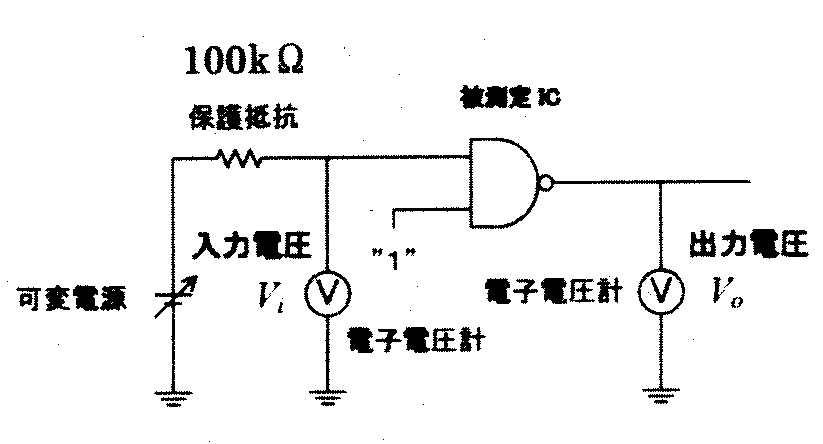
\includegraphics[height=40mm]{実験テキスト/図7.png}
    \caption{IC 74HC00の回路}
  \end{minipage}
  \begin{minipage}{0.5\hsize}
    \centering
    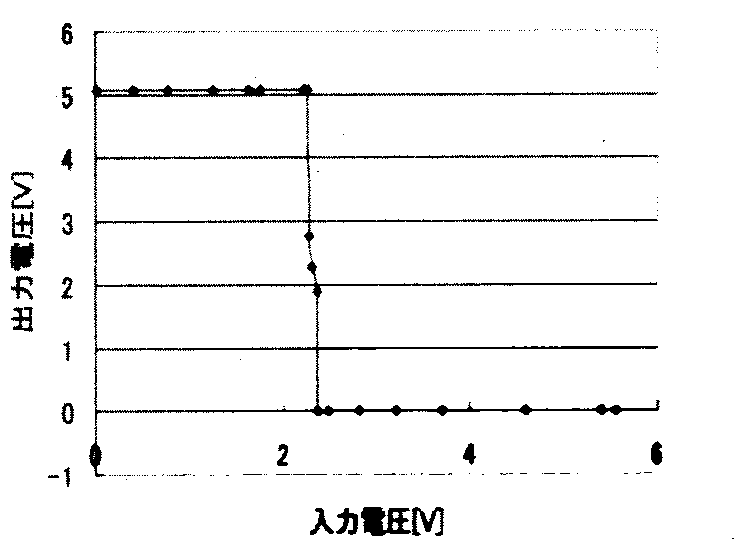
\includegraphics[height=40mm]{実験テキスト/図8.png}
    \caption{IC 74HC00の端子接続図}
  \end{minipage}
\end{figure}
$V_{cc}$または0Vに近い電圧値HまたはLの意味は,図8に示した論理特性が変化しない範囲の電圧値を示している.
これらの値は製品のばらつきのために個々のICによって多少異なるが,標準のCMOSIC($V_{cc}$=5V)では入力電圧に関してLは1.5V以下そして3.5V以上,出力電圧に反してLは0.05V以下そしてHは4.95V以上と規定されている.
入力電圧$V_i$によって出力電圧$V_o$の値が急に変化するところの入力電圧の値を閾値(threshoud level)といい,$V_s$で表す.この測定例では$V_s$=2.4Vである.

\subsection{出力特性の測定}
\begin{wrapfigure}{r}{70mm}
 \vspace*{-\intextsep}
 \begin{center}
  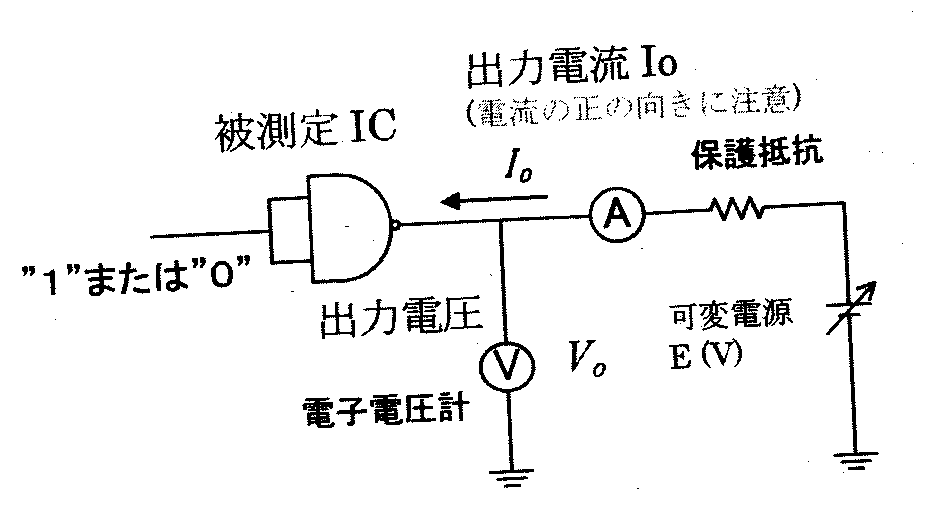
\includegraphics[height=40mm,  angle=-2]{実験テキスト/図9.png}
  \caption{出力特性測定回路}
 \end{center}
\end{wrapfigure}

入力特性はFETのゲート電流は流れないので,CMOSでは0である.
出力特性は図9に示す測定回路により測定でき,その測定例を図10に示す.出力特性を図9に従って出力電流測定する.

その結果より,出力抵抗を求める.
さらに,出力電圧がCMOS規格を満足する条件下での最大出力電流を求める.
出力特性より出力抵抗を求めてみると入力が0Vのときは約50$\Omega$,$V_{cc}$のときは約100$\Omega$であることが得られる.
\begin{figure}[H]
  \centering
  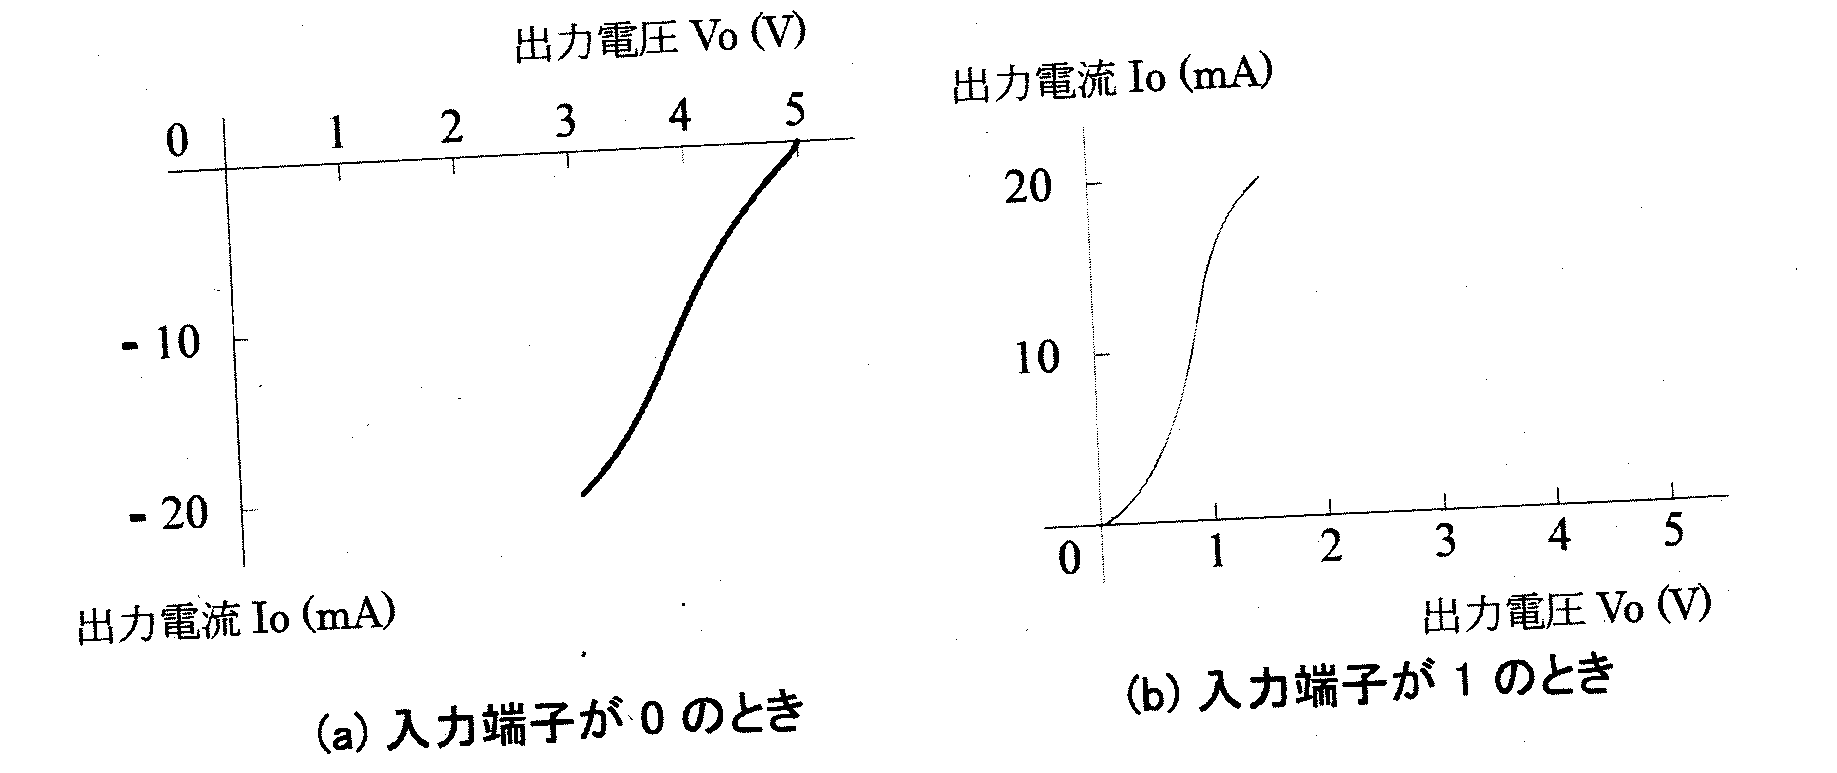
\includegraphics[height=60mm, angle=-3]{実験テキスト/図10.png}
  \caption{出力特性}
\end{figure}

入力特性及び出力特性は互いに密接に関連した意味を持っている.なぜならば,1個のICで何個まで負荷ICを駆動できるかが決まるからである.
この最大負荷数のことをファンアウト数という.CMOSの場合にはTTLと異なり入力電流がほとんど流れないため,ファンアウトを考える必要はない.
しかし,ゲートを複数段接続すると負荷されるコンデンサ容量が大きくなり,その充放電時間が長くなる.
そこで,保証されているファンアウト数は50までであり+,容量負荷では500pFまでである.

一方,TTLを負荷として接続する場合は最大出力電流が問題となる(CMOSよびTTLの入出力電圧規格を参照すると,CMOSを直接TTL入力に接続しても問題ないことが確認できる).
今回の実験試料であるTC74HC00APはLSTTLを直接10個駆動可能となっている.

\newpage
\subsection{非安定性マルチバイブレータの特性測定}
\begin{wrapfigure}{r}{70mm}
 \vspace*{-\intextsep}
 \begin{center}
  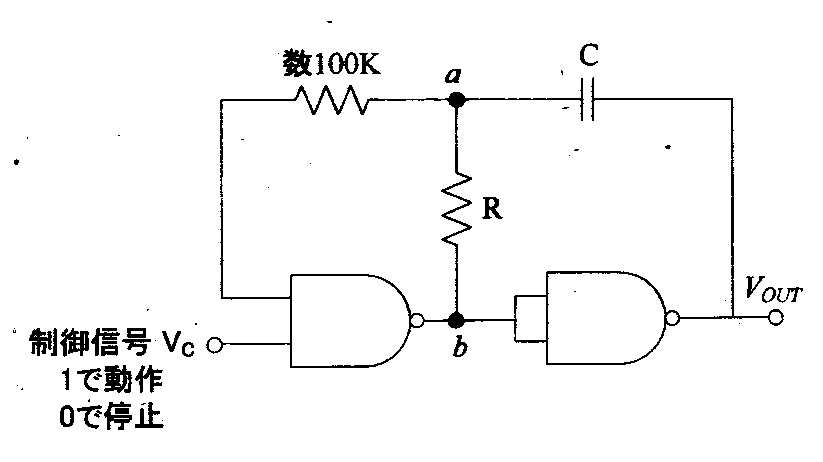
\includegraphics[height=40mm]{実験テキスト/図11.png}
  \caption{非安定マルチバイブレータ}
  \label{fig:図11}
 \end{center}
\end{wrapfigure}
一般に2変数NANDまたはNORゲートなどだけでいかなる論理特性をも実現できることはキロン的に明らかにされているので,74HC00によって任意の機能を持つ回路を実現できる.
ここでは,マルチバイブレータについて考えてみよう.
マルチバイブレータには双安定形(実はflip flopのこと),単安定形(monostable multivibratorまたはoneshot multivibrator)および非安定形(astable multivibrator これをマルチバイブレータと呼ぶこともある)があるが,非安定マルチバイブレータについて考えてみる.
回路の一例を図11に示す.
制御信号$V_c$によって発振を制御できる.
発振周期Tは次式により決定できる.
\begin{equation}
T \approx 2CR \log_e \{ (V_H + V_S) / V_S \} = 2CR \ln \{ (V_H + V_S) / V_S \}
\end{equation}
$V_H$および$V_S$は,図8に示したようにそれぞれ$V_i$=0としたときの出力電圧$V_H$および理論値の変化するところの入力電圧すなわち閾値$V_S$である.

図11の非安定マルチバイブレータの各部の波形を観測し,周期を測定する.
数種類のCについて同様の実験を行う.

実験を行う上で,以下の点に注意し実験を行うこと.
\begin{enumerate}
\item 試料74HC00には4個のNAND素子が入っているが,配線の容易なものを選ぶこと.
\item 各ICの電源電圧は必ず定格値5Vに保持し,また入力電圧も5Vを超えないように注意すること.
	過大に加えたりすると破壊される.
	端子位置特に電源端子の位置に十分注意すること.
	ICをソケットに挿入する方向を間違わないこと.
\item 今後の回路制作のためにも,各ICにおいて電源と接地端子間にはバイパスコンデンサを接続しておくこと.
\end{enumerate}

\newpage
\section{結果の処理}
\subsection{電源電流特性(貫通電流特性)の測定}
3.1に示した実験の測定値を表\ref{tbl:3.1}に,測定値をもとに入力電圧と電源電流の関係を図\ref{fig:3.1}に示す.
\begin{figure}[H]
	\begin{tabular}{cc}
		\begin{minipage}{0.33\hsize}
			\tblcaption{測定値}
			\label{tbl:3.1}
			\centering
			\small
			\begin{tabular}{|r|r|}\hline
				入力電圧[V] & 電源電流[mA] \\\hline
				0.002  & 0.050  \\\hline
				0.200  & 0.050  \\\hline
				0.398  & 0.050  \\\hline
				0.610  & 0.050  \\\hline
				0.811  & 0.055  \\\hline
				1.011  & 0.110  \\\hline
				1.203  & 0.282  \\\hline
				1.308  & 0.420  \\\hline
				1.356  & 0.516  \\\hline
				1.400  & 0.598  \\\hline
				1.446  & 0.680  \\\hline
				1.502  & 0.792  \\\hline
				1.558  & 0.910  \\\hline
				1.607  & 1.040  \\\hline
				1.710  & 1.290  \\\hline
				1.802  & 1.504  \\\hline
				1.900  & 1.800  \\\hline
				1.953  & 1.990  \\\hline
				2.011  & 2.200  \\\hline
				2.053  & 2.440  \\\hline
				2.108  & 3.200  \\\hline
				2.156  & 12.400  \\\hline
				2.202  & 12.400  \\\hline
				2.305  & 12.300  \\\hline
				2.404  & 12.300  \\\hline
				2.505  & 12.200  \\\hline
				2.601  & 12.100  \\\hline
				2.707  & 11.500  \\\hline
				2.747  & 1.800  \\\hline
				2.808  & 1.630  \\\hline
				2.911  & 1.490  \\\hline
				3.015  & 1.250  \\\hline
				3.302  & 0.790  \\\hline
				3.612  & 0.380  \\\hline
				3.709  & 0.170  \\\hline
				3.818  & 0.100  \\\hline
				3.915  & 0.050  \\\hline
				4.009  & 0.020  \\\hline
				4.520  & 0.000  \\\hline
				5.060  & 0.000  \\\hline
			\end{tabular}
			\normalsize
		\end{minipage}
		\begin{minipage}{0.66\hsize}
			\centering
			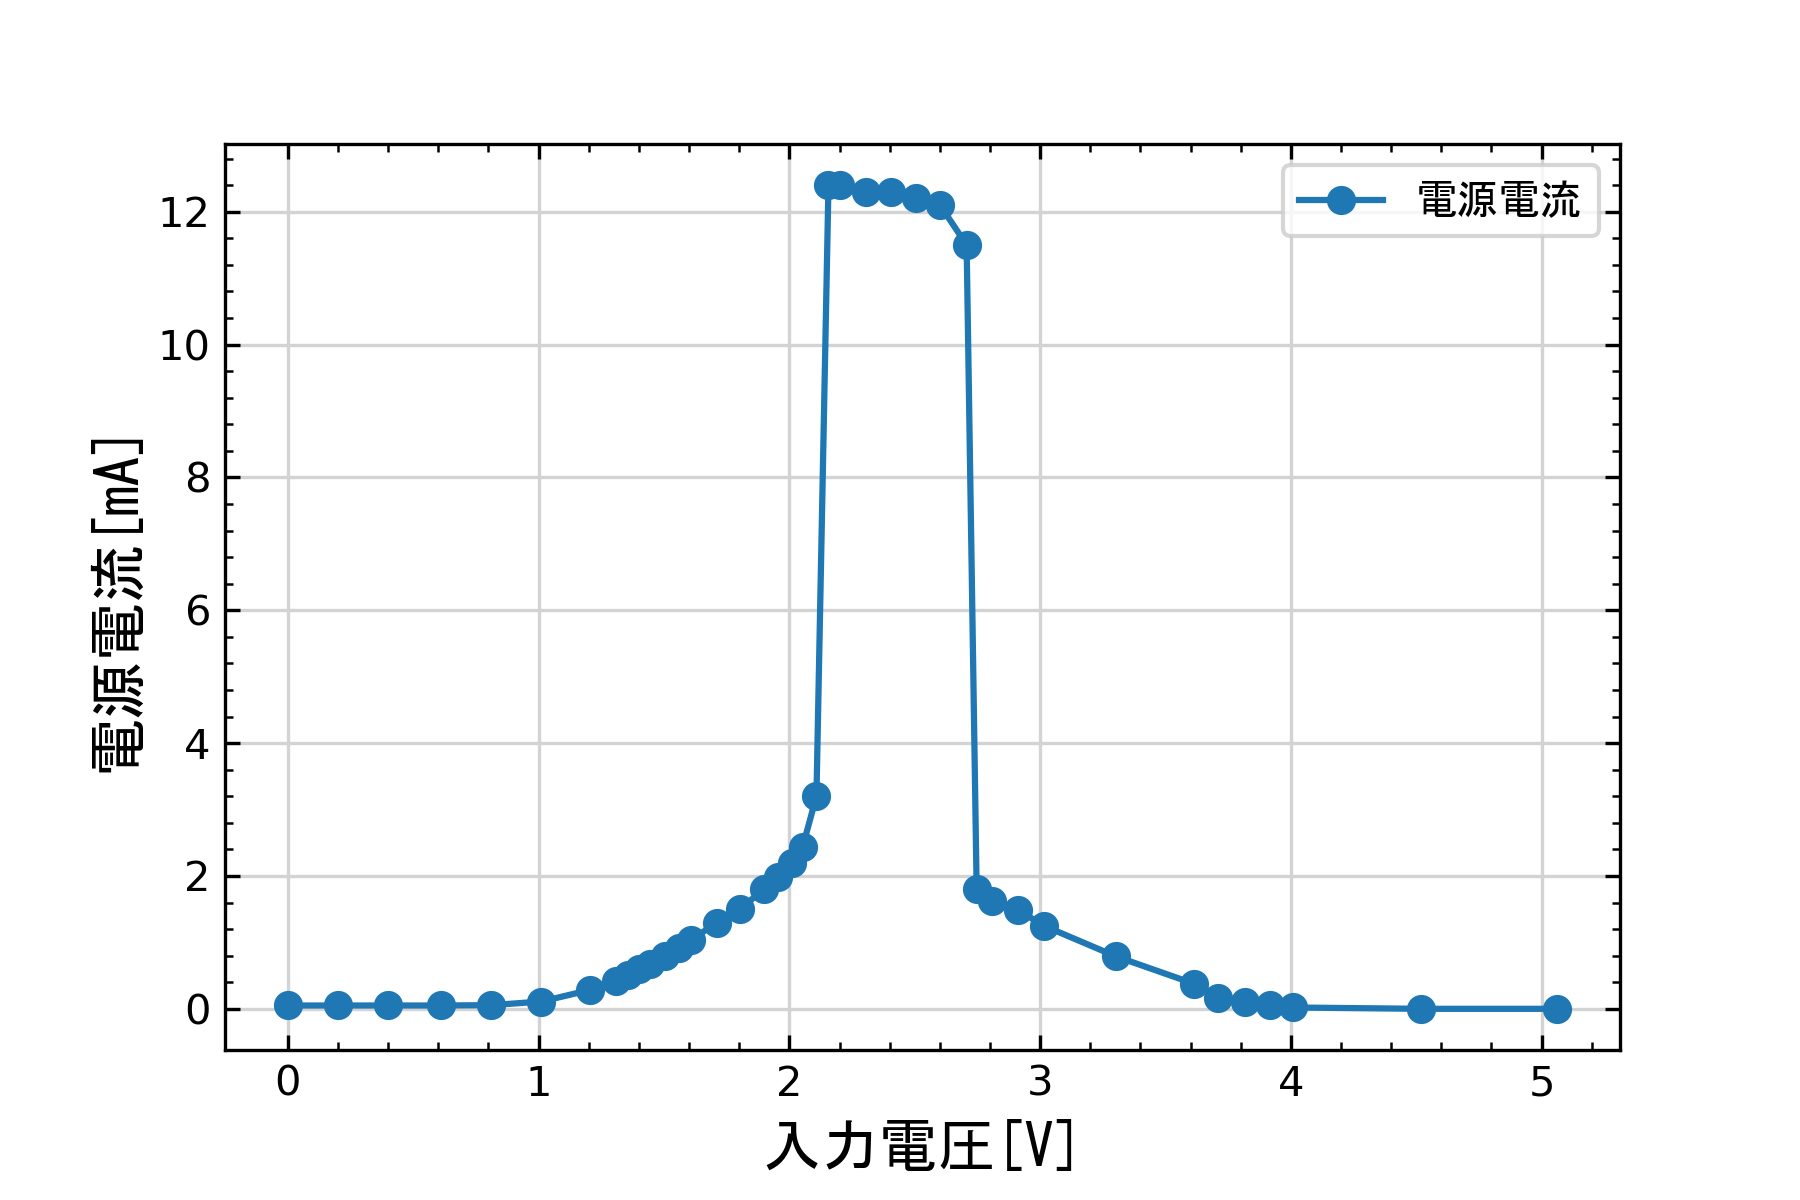
\includegraphics[width = \hsize]{Result/Experiment/実験3_1.png}
			\figcaption{測定した電源電流特性}
			\label{fig:3.1}
		\end{minipage}
	\end{tabular}
\end{figure}

\newpage
\subsection{入出力伝達特性の測定}
3.2に示した実験の測定値を表\ref{tbl:3.2}に,測定値をもとに入力電圧と出力電圧の関係を図\ref{fig:3.2}に示す.
\begin{figure}[H]
	\begin{tabular}{cc}
		\begin{minipage}{0.33\hsize}
			\tblcaption{測定値}
			\label{tbl:3.2}
			\centering
			\small
			\begin{tabular}{|r|r|}\hline
				入力電源[V] & 出力電源[V] \\\hline
				0.000  & 4.98  \\\hline
				0.198  & 4.99  \\\hline
				0.409  & 5.00  \\\hline
				0.602  & 5.00  \\\hline
				0.803  & 5.00  \\\hline
				1.007  & 5.00  \\\hline
				1.202  & 5.00  \\\hline
				1.404  & 5.00  \\\hline
				1.608  & 5.00  \\\hline
				1.802  & 4.99  \\\hline
				2.007  & 4.98  \\\hline
				2.107  & 4.80  \\\hline
				2.117  & 2.21  \\\hline
				2.151  & 2.17  \\\hline
				2.208  & 1.98  \\\hline
				2.252  & 1.83  \\\hline
				2.302  & 1.75  \\\hline
				2.353  & 1.59  \\\hline
				2.400  & 1.40  \\\hline
				2.454  & 1.19  \\\hline
				2.505  & 1.05  \\\hline
				2.550  & 0.00  \\\hline
				2.601  & 0.00  \\\hline
				2.809  & 0.00  \\\hline
				3.001  & 0.00  \\\hline
				3.507  & 0.00  \\\hline
				4.007  & 0.00  \\\hline
				4.500  & 0.00  \\\hline
				5.006  & 0.00  \\\hline
			\end{tabular}
			\normalsize
		\end{minipage}
		\begin{minipage}{0.66\hsize}
			\centering
			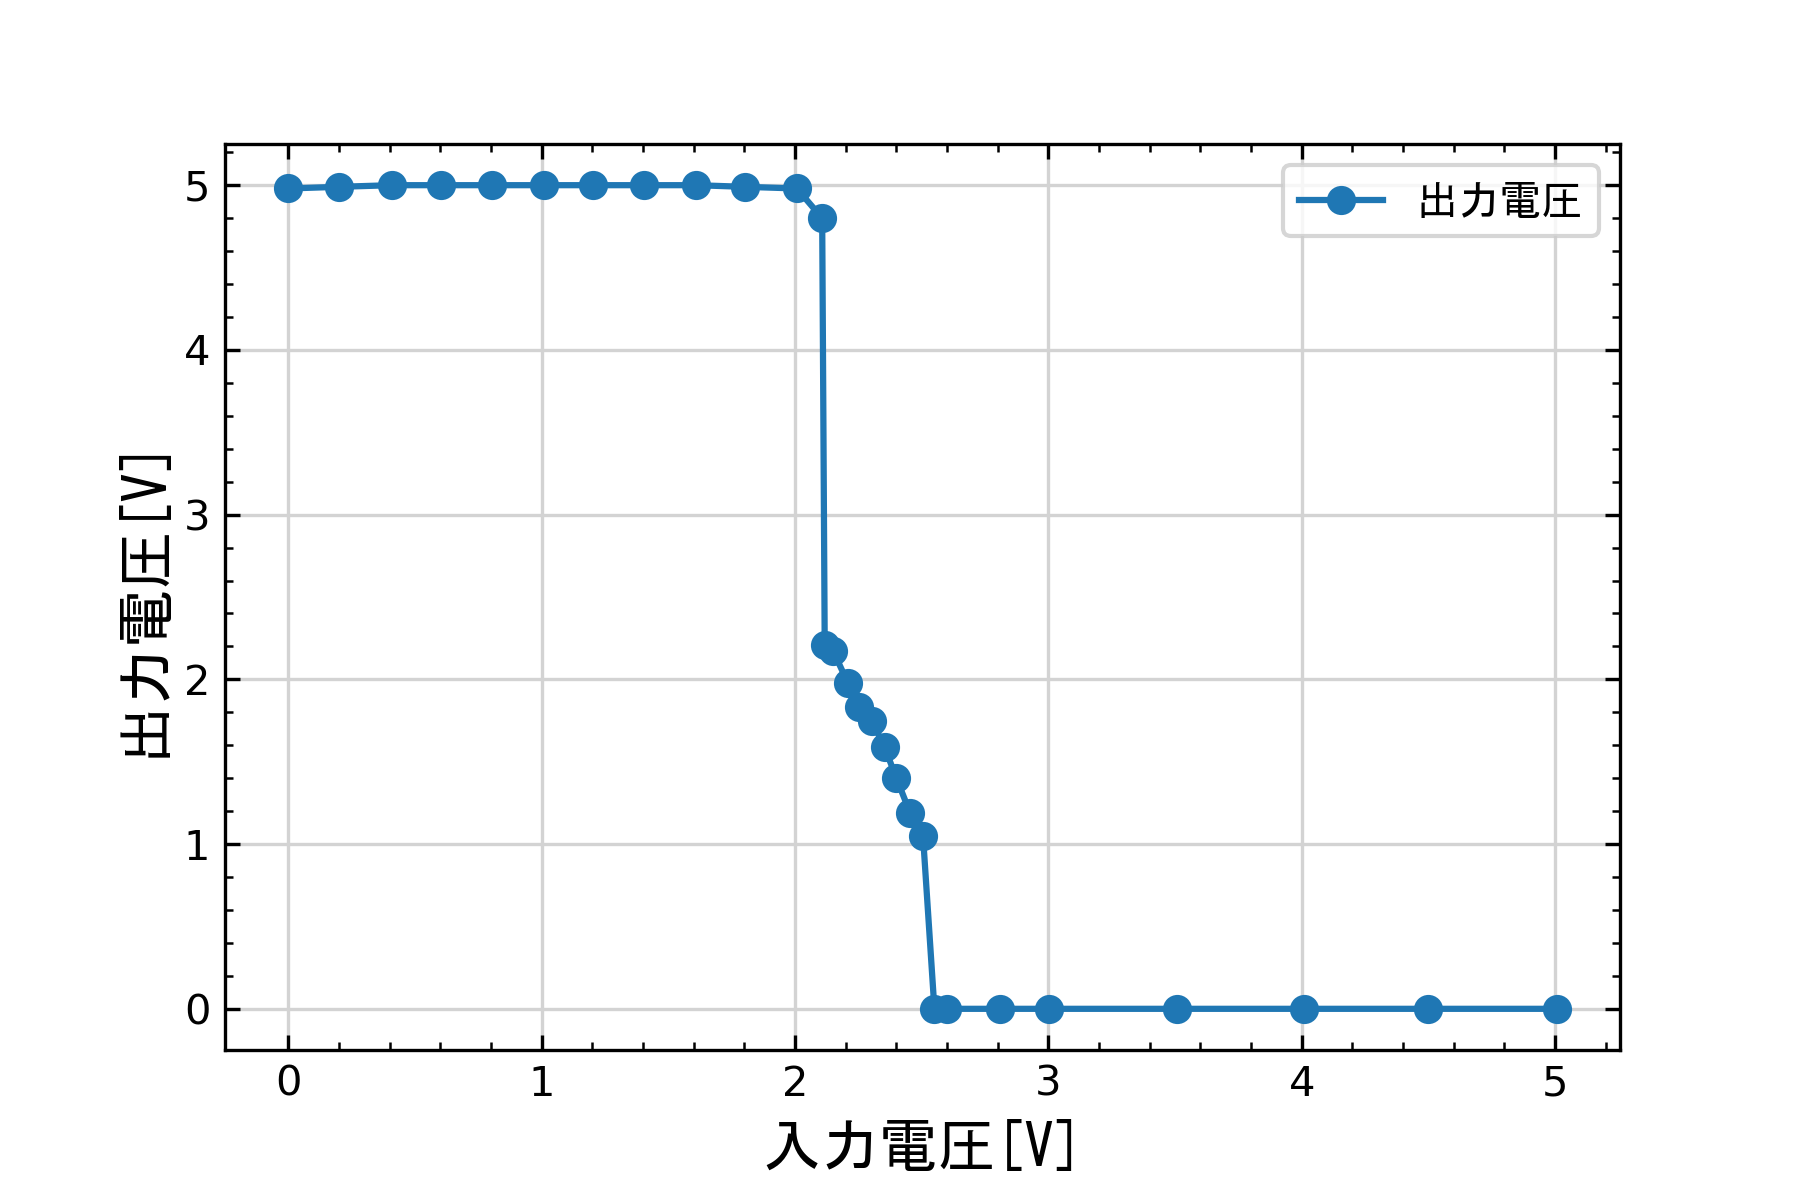
\includegraphics[width = \hsize]{Result/Experiment/実験3_2.png}
			\figcaption{測定した入出力伝達特性}
			\label{fig:3.2}
		\end{minipage}
	\end{tabular}
\end{figure}

\newpage
\subsection{出力特性の測定}
3.3に示した実験の測定値を出力の条件ごとに表\ref{tbl:3.3-0},表\ref{tbl:3.3-1}に,測定値をもとに出力電流と出力電圧の関係をそれぞれ図\ref{fig:3.3-0},図\ref{fig:3.3-1}に示す.
\begin{figure}[H]
	\begin{tabular}{cc}
		\begin{minipage}{0.33\hsize}
			\tblcaption{測定値}
			\label{tbl:3.3-0}
			\centering
			\small
			\begin{tabular}{|r|r|}\hline
				出力電圧[V] & 出力電流[mA] \\\hline
				5.000  & -0.560  \\\hline
				4.980  & -1.180  \\\hline
				4.960  & -1.600  \\\hline
				4.940  & -2.240  \\\hline
				4.920  & -2.620  \\\hline
				4.900  & -3.180  \\\hline
				4.880  & -3.780  \\\hline
				4.860  & -4.280  \\\hline
				4.840  & -4.650  \\\hline
				4.820  & -5.210  \\\hline
				4.800  & -5.650  \\\hline
				4.780  & -6.190  \\\hline
				4.760  & -6.700  \\\hline
				4.740  & -7.180  \\\hline
				4.720  & -7.700  \\\hline
				4.700  & -8.200  \\\hline
			\end{tabular}
			\normalsize
		\end{minipage}
		\begin{minipage}{0.66\hsize}
			\centering
			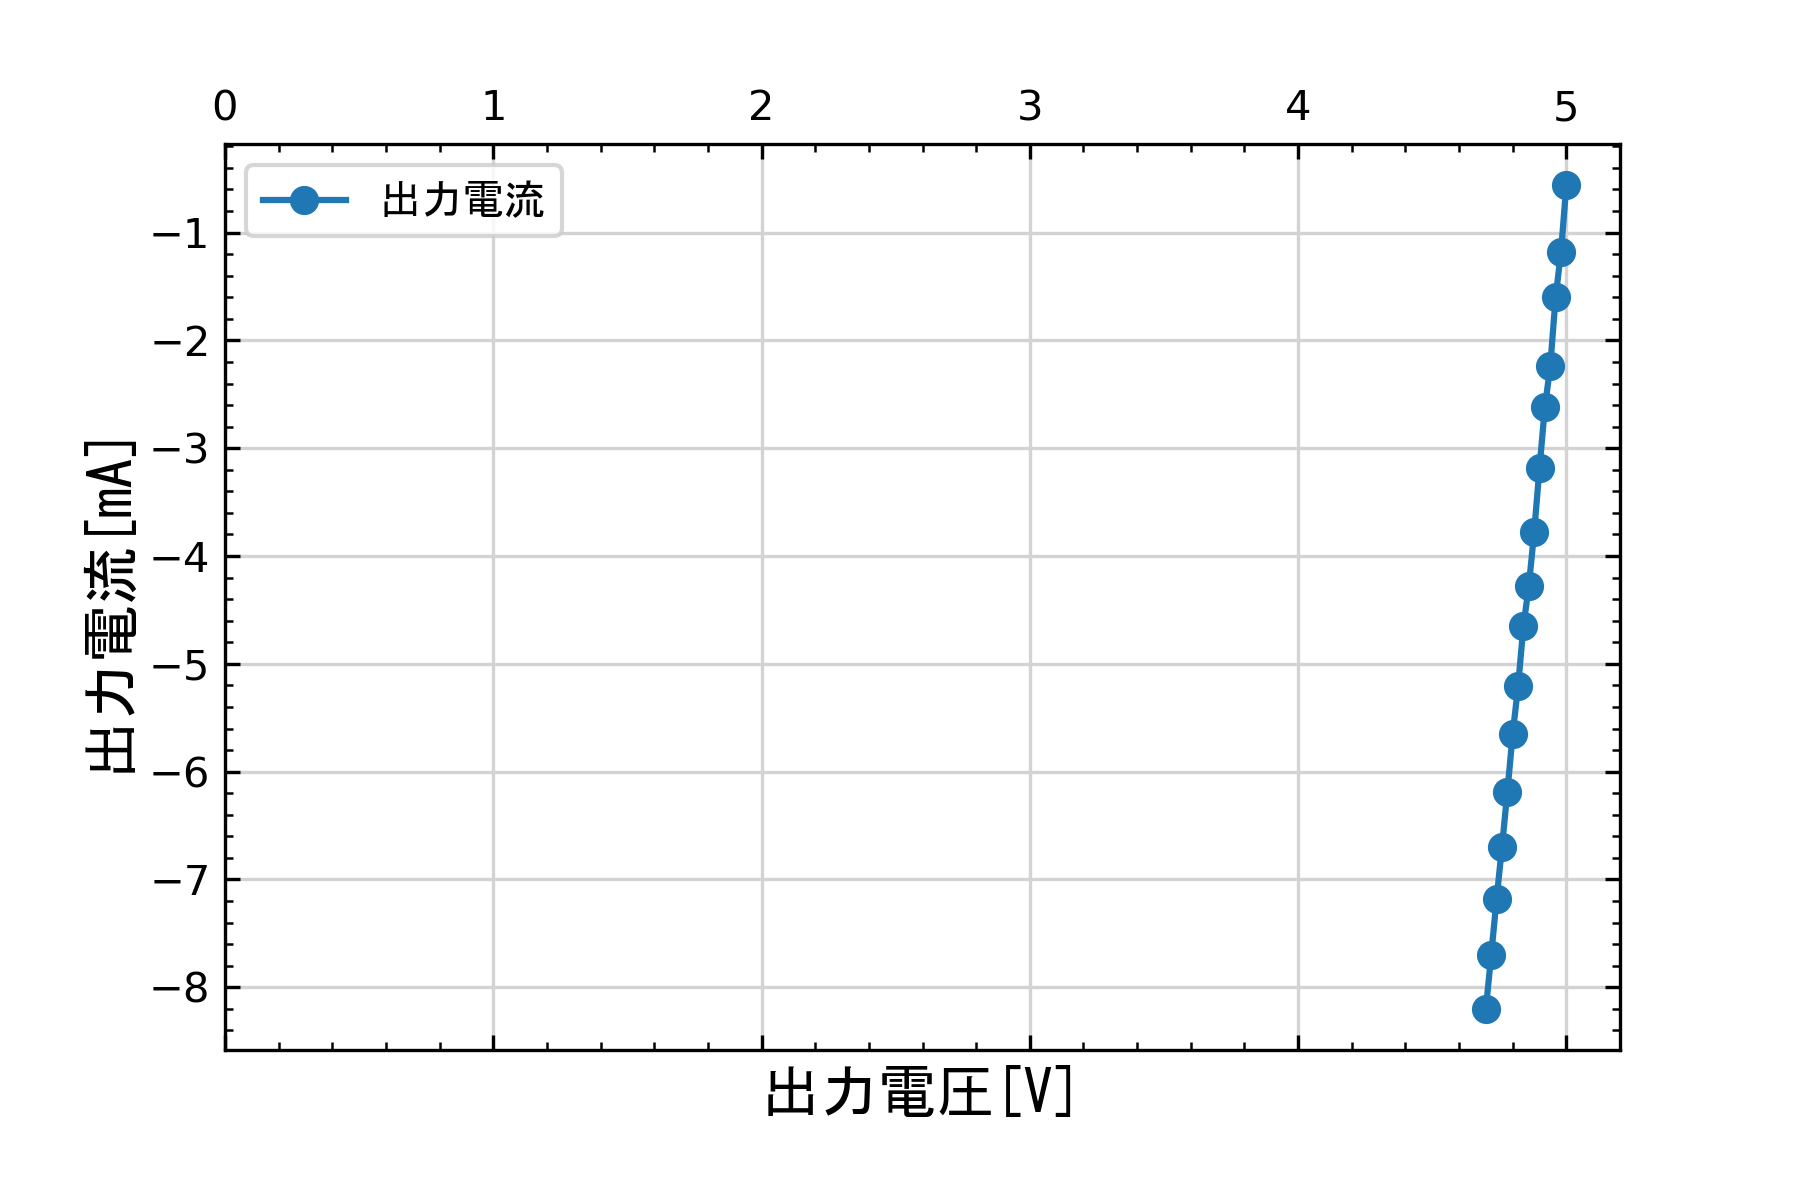
\includegraphics[width = \hsize]{Result/Experiment/実験3_3.png}
			\figcaption{測定した出力特性}
			\label{fig:3.3-0}
		\end{minipage}
	\end{tabular}
	\centering \\*
	出力0のとき
\end{figure}
\begin{figure}[H]
	\begin{tabular}{cc}
		\begin{minipage}{0.33\hsize}
			\normalsize
			\tblcaption{測定値}
			\label{tbl:3.3-1}
			\centering
			\small
			\begin{tabular}{|r|r|}\hline
				出力電圧[V] & 出力電流[mA] \\\hline
				0.000  & 0.000  \\\hline
				0.100  & 3.490  \\\hline
				0.200  & 6.721  \\\hline
				0.300  & 10.000  \\\hline
				0.400  & 12.607  \\\hline
				0.500  & 16.100  \\\hline
				0.600  & 18.883  \\\hline
				0.700  & 22.600  \\\hline
				0.800  & 23.667  \\\hline
				0.900  & 25.900  \\\hline
				1.000  & 27.821  \\\hline
			\end{tabular}
			\normalsize
		\end{minipage}
		\begin{minipage}{0.66\hsize}
			\centering
			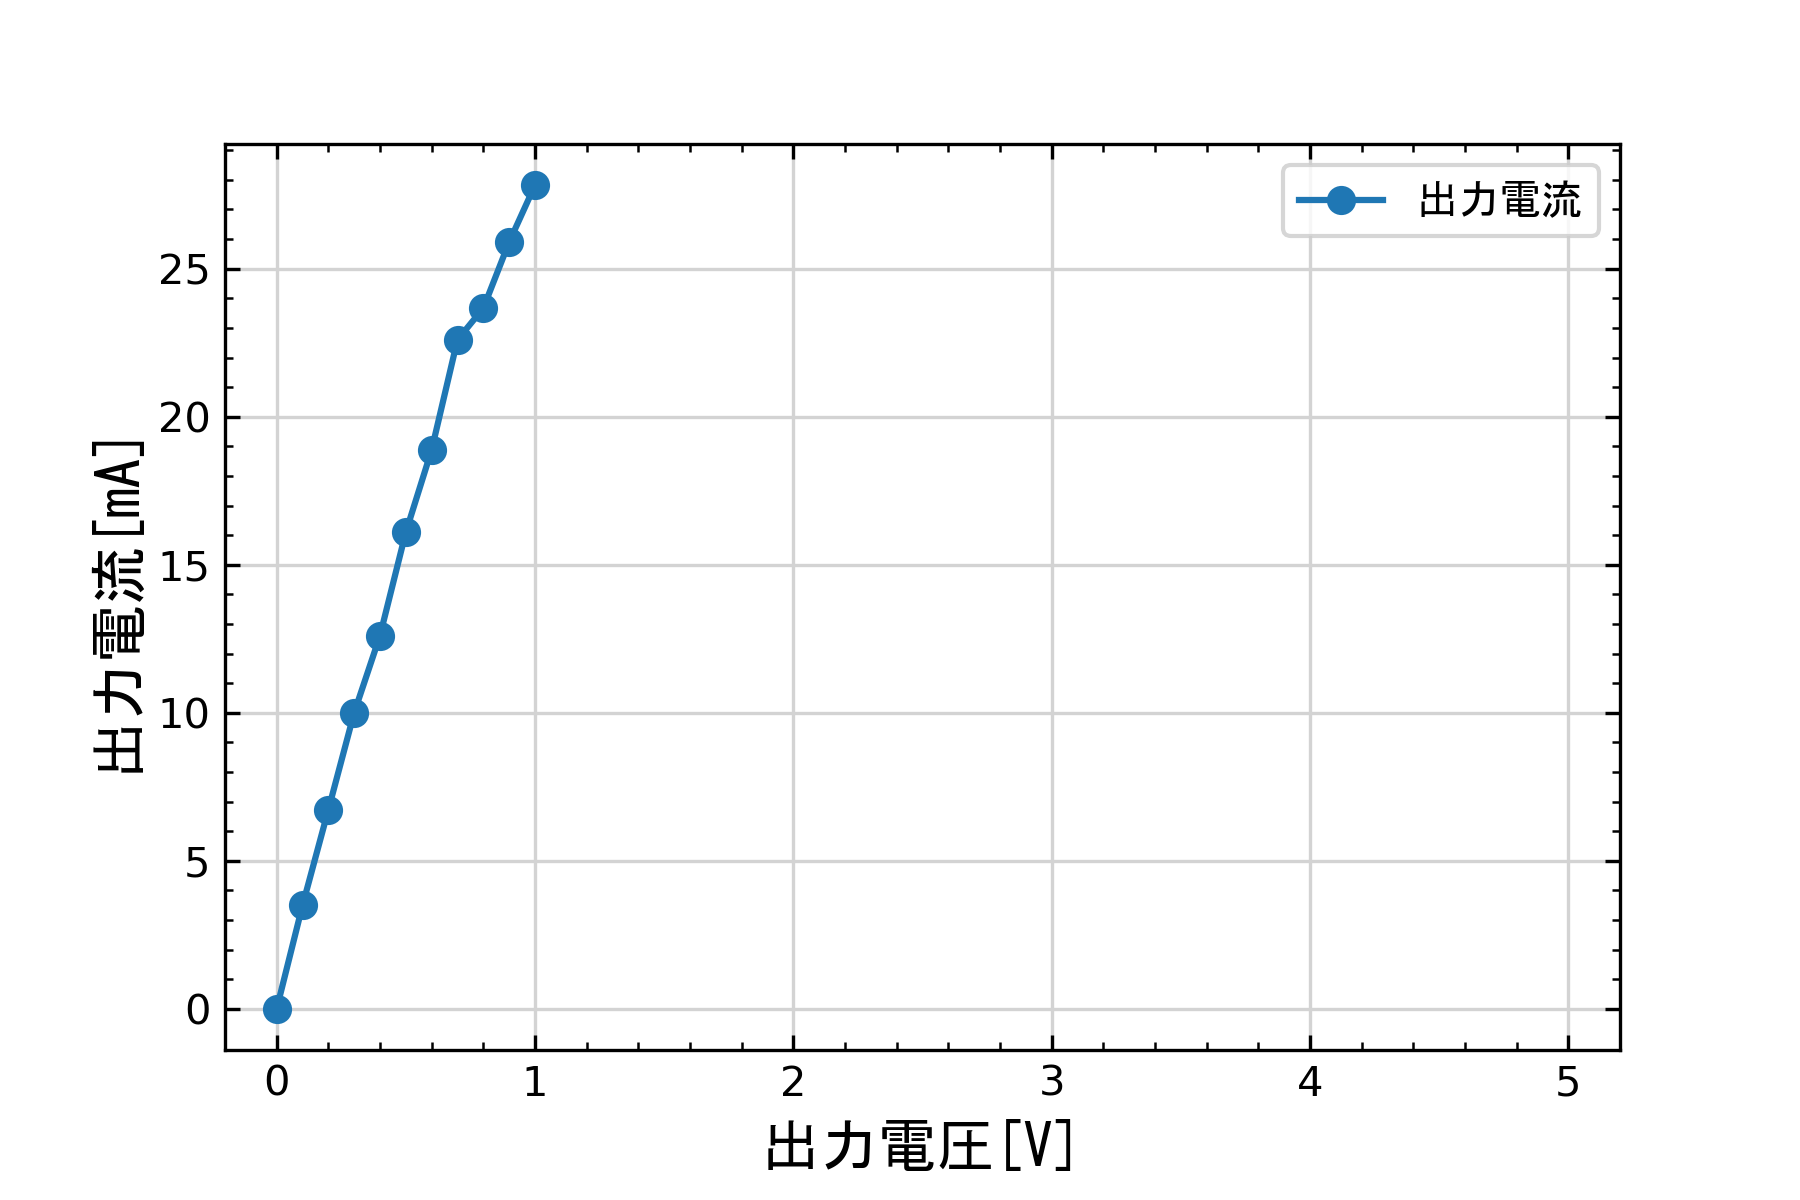
\includegraphics[width = \hsize]{Result/Experiment/実験3_4.png}
			\figcaption{測定した出力特性}
			\label{fig:3.3-1}
		\end{minipage}
	\end{tabular}
	\centering \\*
	出力1のとき
\end{figure}

\newpage
\subsection{非安定マルチバイブレータの特性}
3.4に示した実験の結果を以下の図に示す.また,実験時に使用したコンデンサを以下の表\ref{tbl:3.4-C}に示す.

\begin{figure}[H]
	\centering
	\tblcaption{コンデンサの値と周期T}
	\label{tbl:3.4-C}
	\begin{tabular}{|c|c|c|}\hline
		& \multicolumn{2}{|c|}{周期 T [ms]}  \\\cline{2-3}
		静電容量C[$\mu$F] & 理論値 & 測定値 \\\hline
		1.000 & 2.197 & 2.4 \\\hline
		0.220 & 0.483 & 0.53 \\\hline
		0.022 & 0.048 & 0.06 \\\hline
	\end{tabular}
\end{figure}

\subsubsection{C = 1[$\mu$F]の時の波形}
以下に図\ref{fig:図11}のCを1.000[$\mu$F]としたときのVout,Va,Vb,Vdの各波形を示す.
\begin{figure}[H]
	\centering
	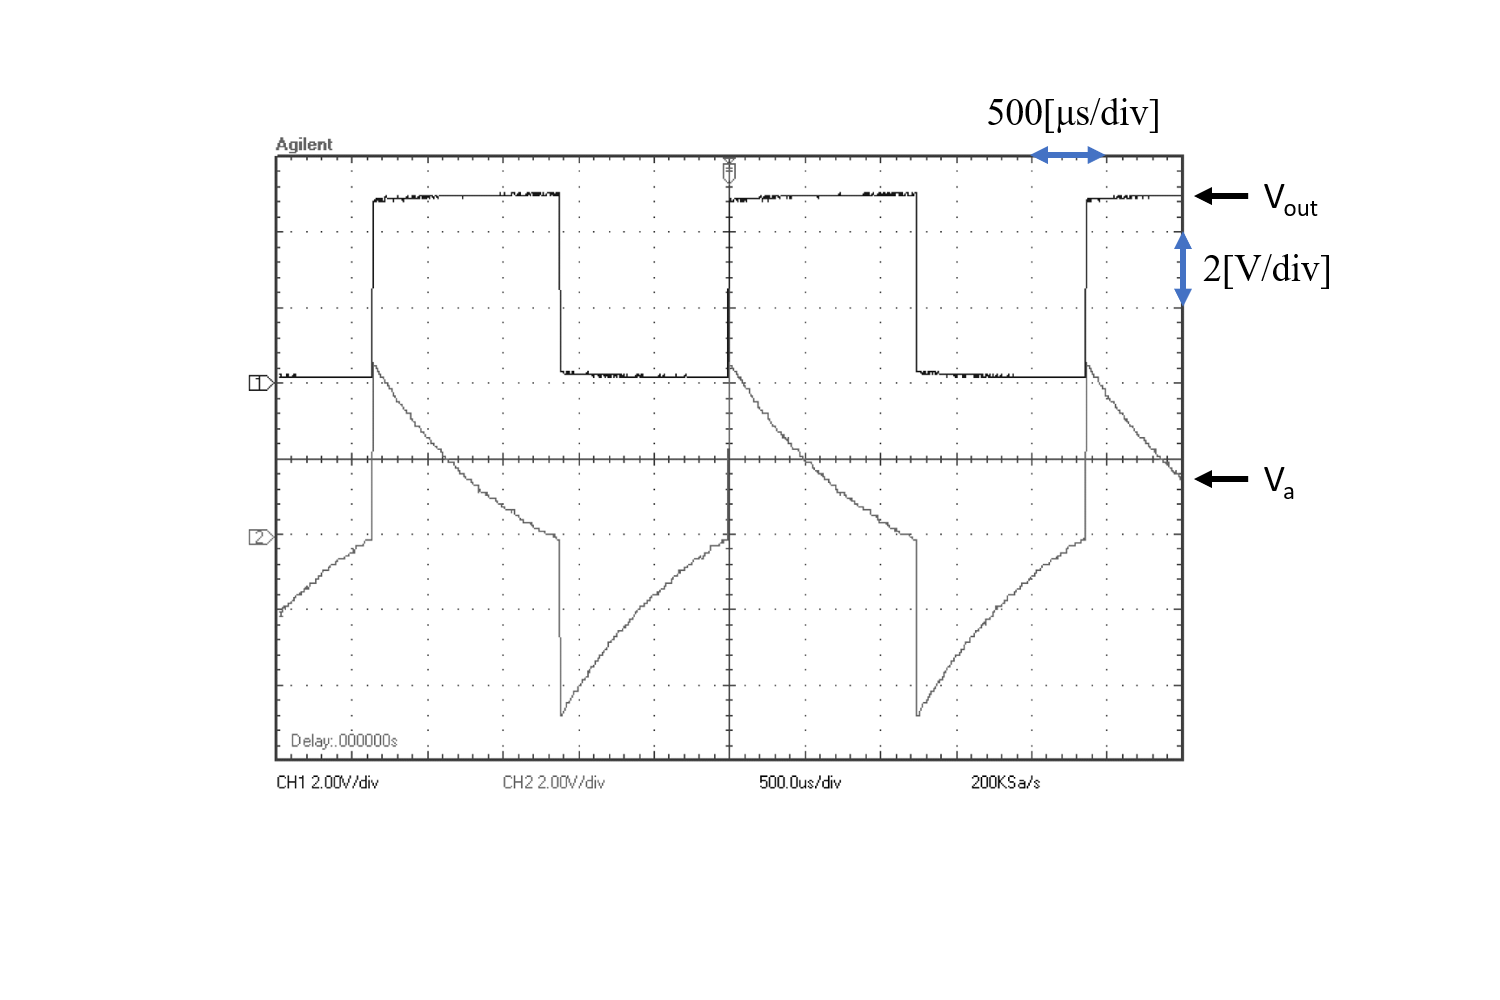
\includegraphics[width=\hsize]{images/r105m-Vout-Va.png}
	\figcaption{Vout,Vaの出力波形}
	\label{r105m-Vout-Va}
\end{figure}
\begin{figure}[H]
	\centering
	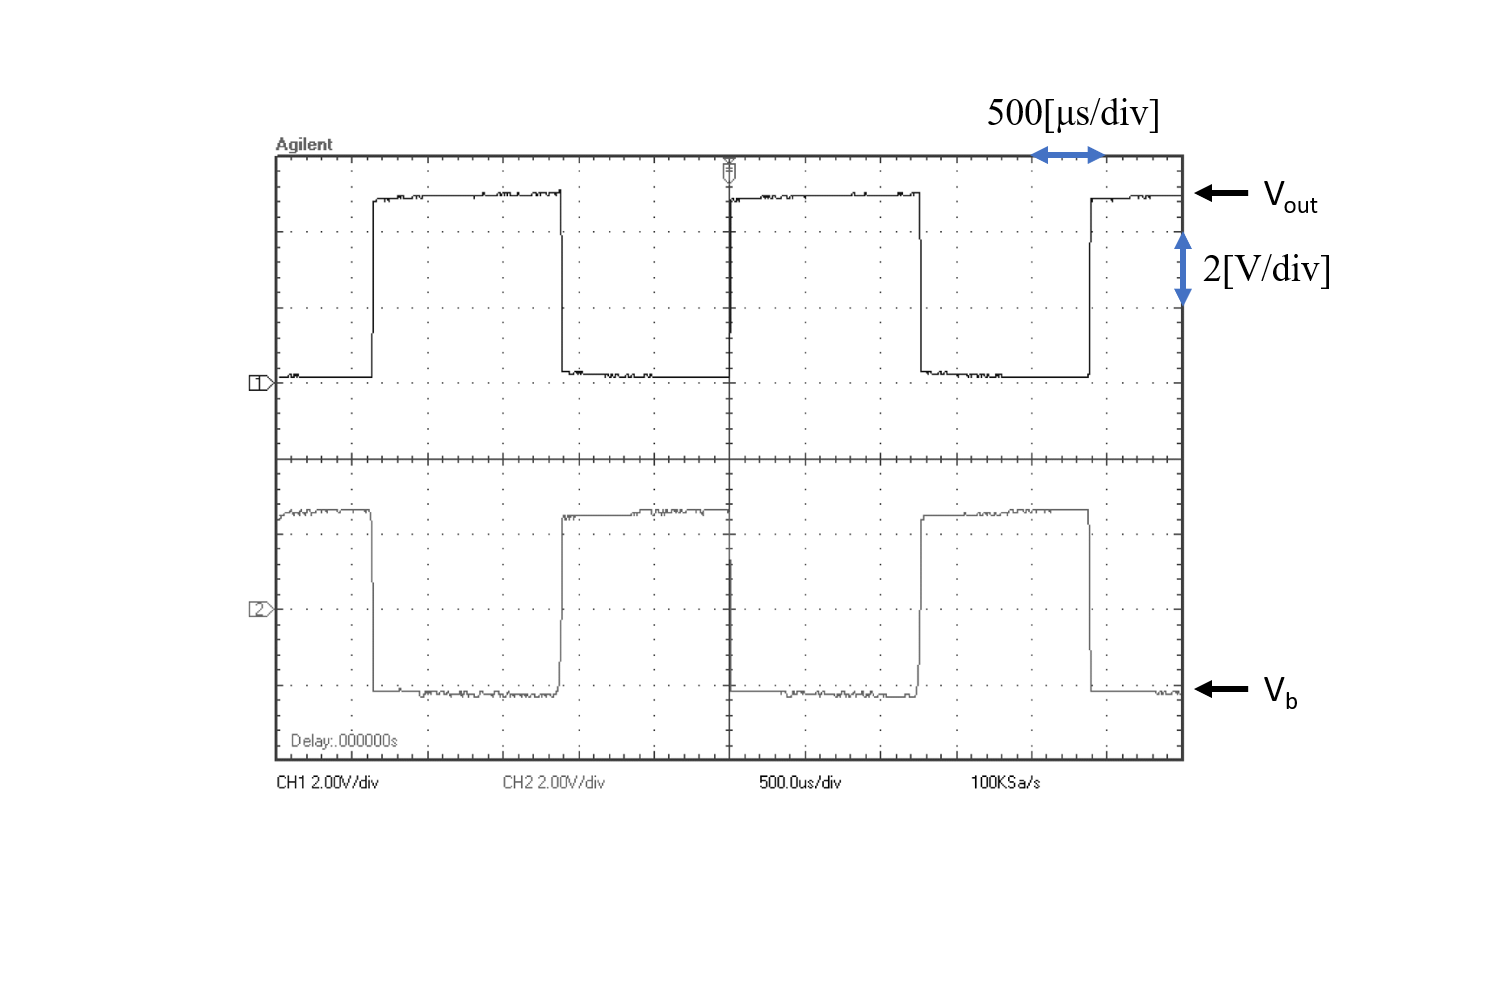
\includegraphics[width=\hsize]{images/r105m-Vout-Vb.png}
	\figcaption{Vout,Vbの出力波形}
	\label{r105m-Vout-Vb}
\end{figure}
\begin{figure}[H]
	\centering
	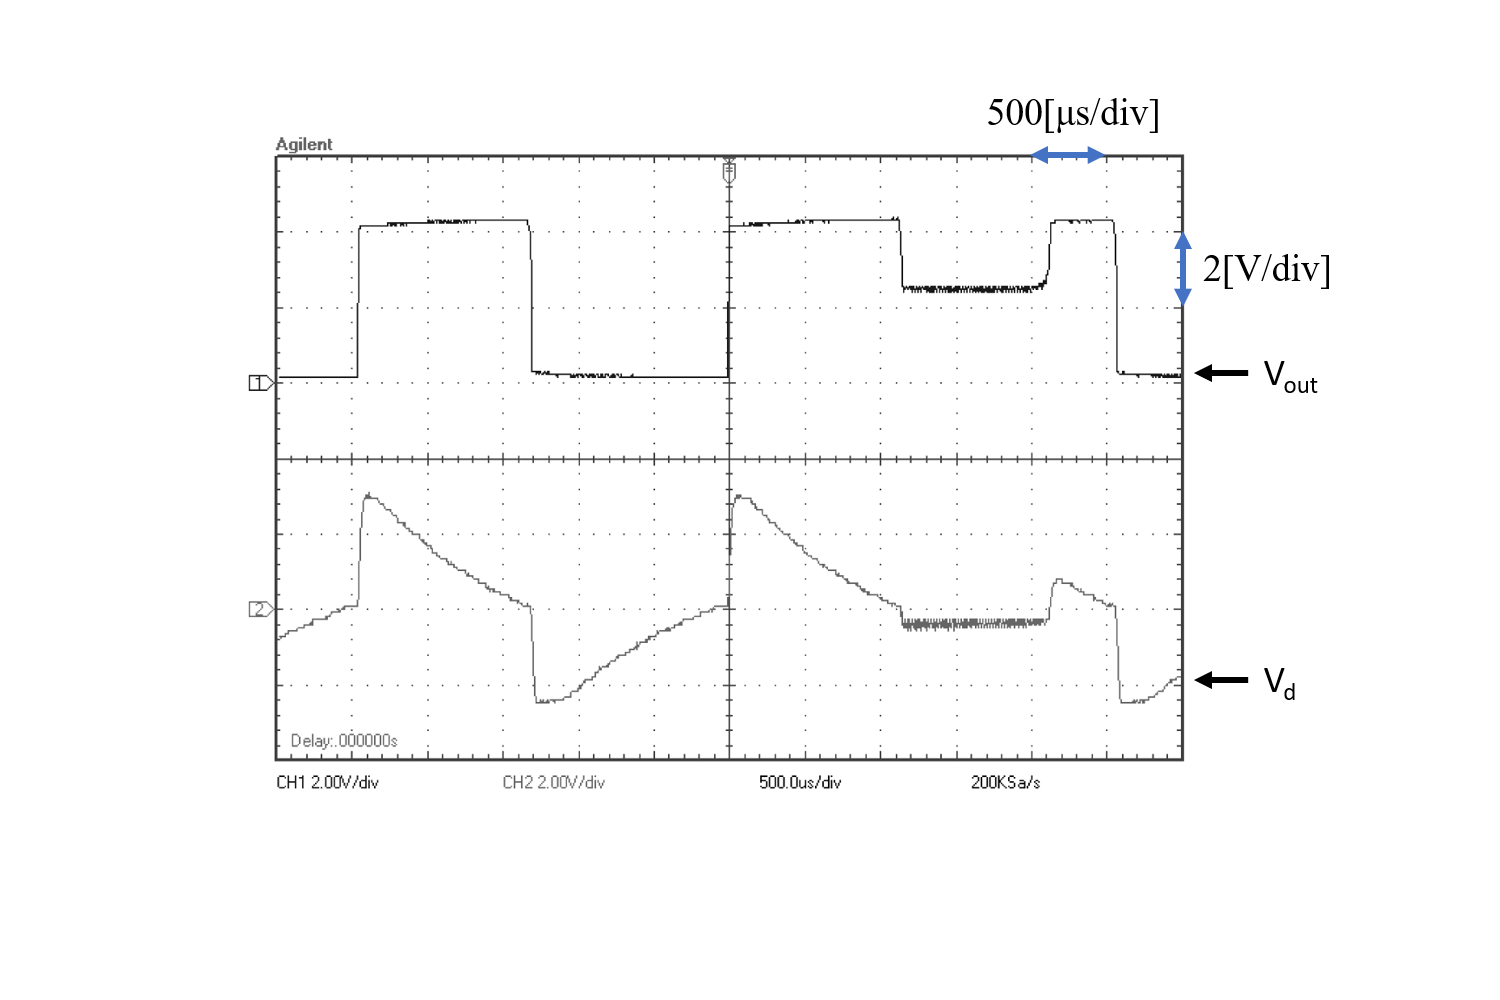
\includegraphics[width=\hsize]{images/r105m-Vout-Vd.png}
	\figcaption{Vout,Vdの出力波形}
	\label{r105m-Vout-Vd}
\end{figure}

\newpage
\subsubsection{C = 0.220[$\mu$F]の時の波形}
以下に図\ref{fig:図11}のCを0.220[$\mu$F]としたときのVout,Va,Vb,Vdの各波形を示す.
\begin{figure}[H]
	\centering
	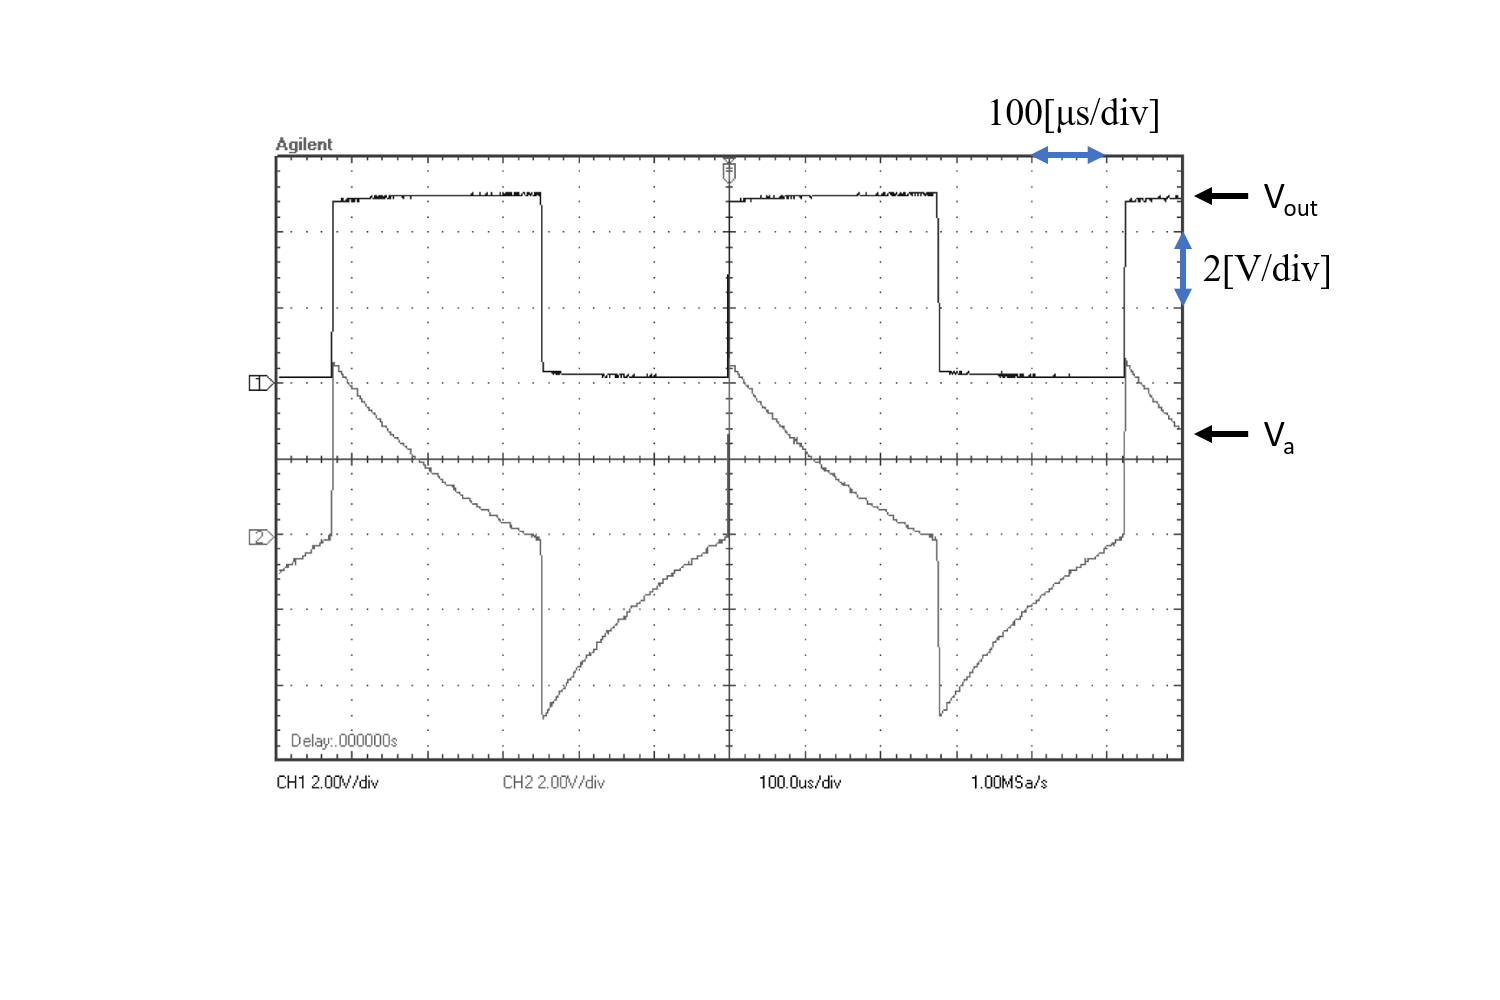
\includegraphics[width=\hsize]{images/224j-Vout-Va.png}
	\figcaption{Vout,Vaの出力波形}
	\label{224j-Vout-Va}
\end{figure}
\begin{figure}[H]
	\centering
	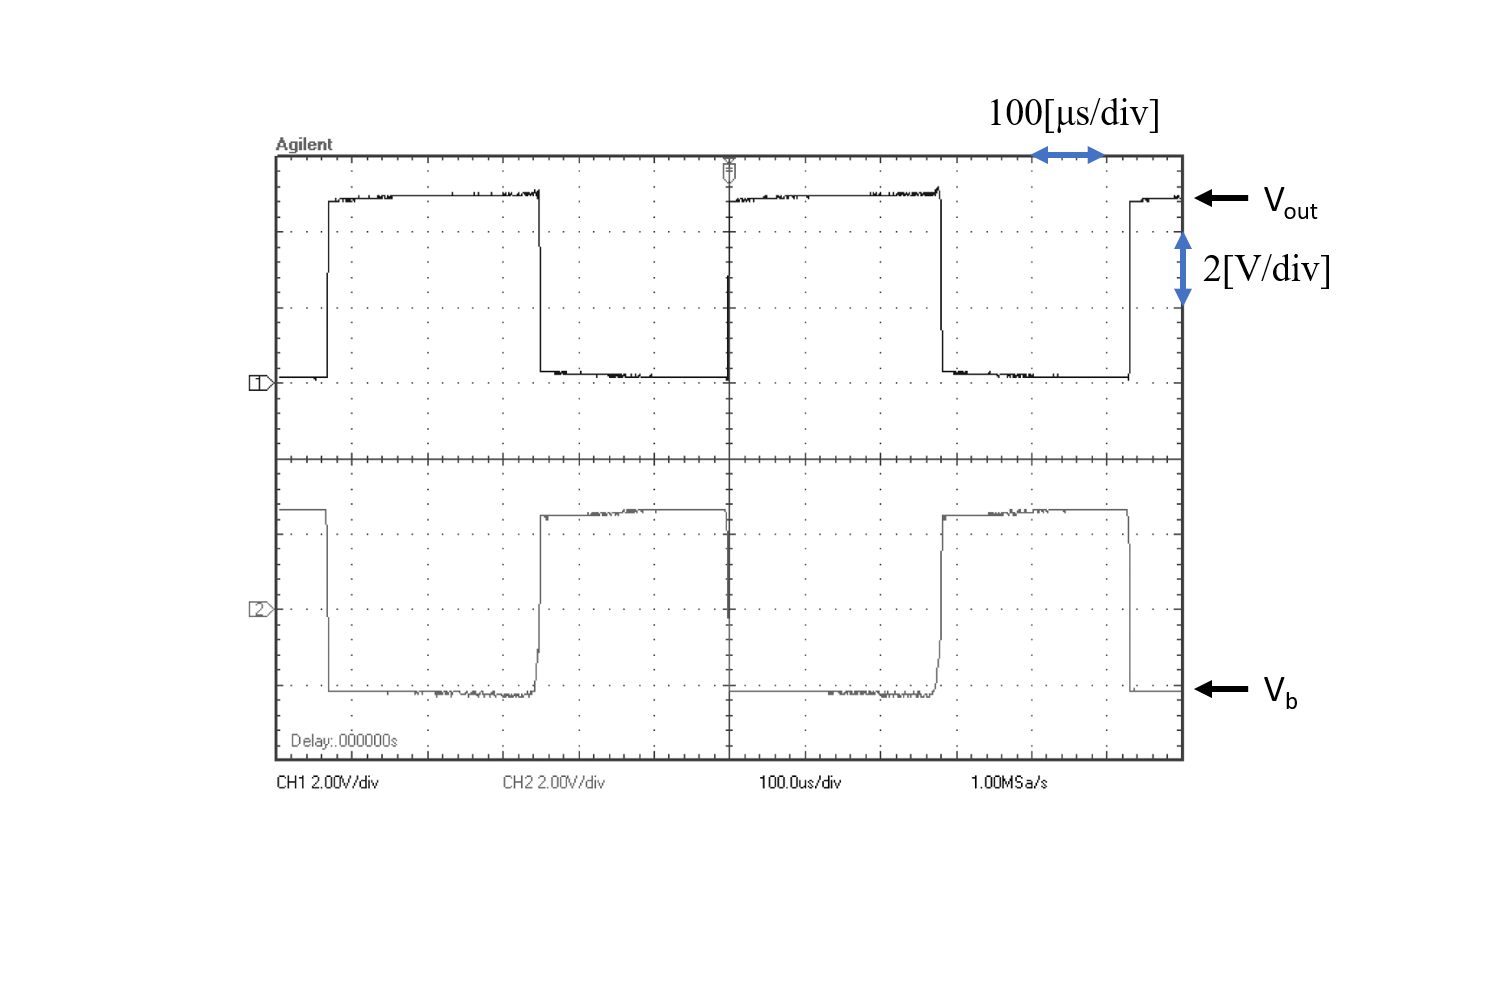
\includegraphics[width=\hsize]{images/224j-Vout-Vb.png}
	\figcaption{Vout,Vbの出力波形}
	\label{224j-Vout-Vb}
\end{figure}
\begin{figure}[H]
	\centering
	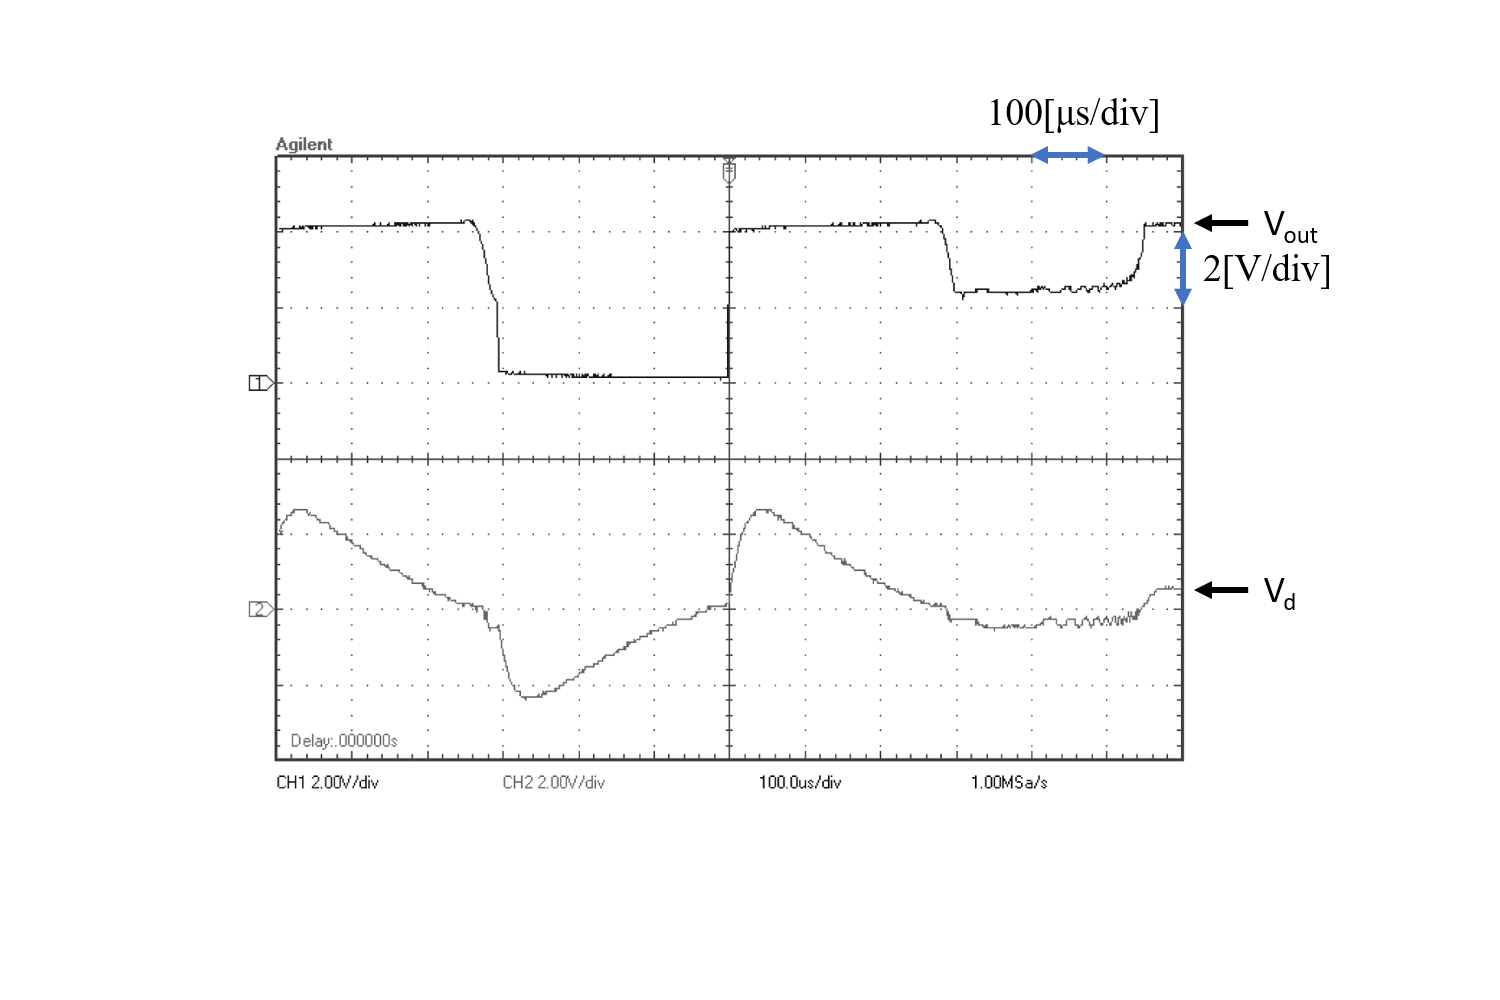
\includegraphics[width=\hsize]{images/224j-Vout-Vd.png}
	\figcaption{Vout,Vdの出力波形}
	\label{224j-Vout-Vd}
\end{figure}

\newpage
\subsubsection{C = 1[$\mu$F]の時の波形}
以下に図\ref{fig:図11}のCを0.022[$\mu$F]としたときのVout,Va,Vb,Vdの各波形を示す.
\begin{figure}[H]
	\centering
	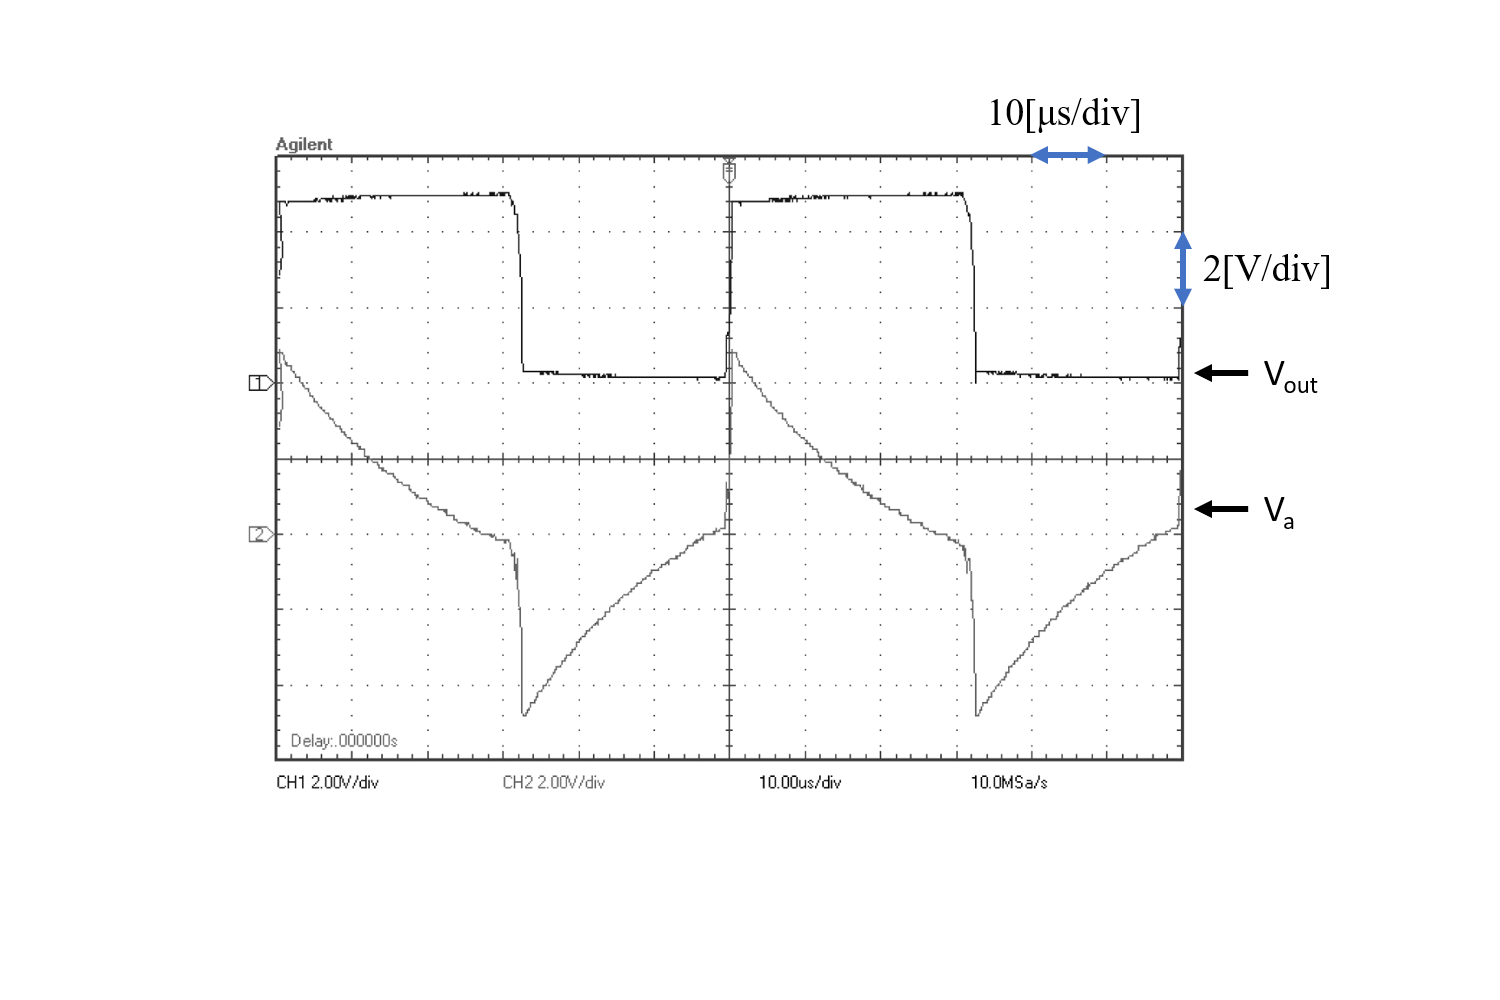
\includegraphics[width=\hsize]{images/223kc-Vout-Va.png}
	\figcaption{Vout,Vaの出力波形}
	\label{223kc-Vout-Va}
\end{figure}
\begin{figure}[H]
	\centering
	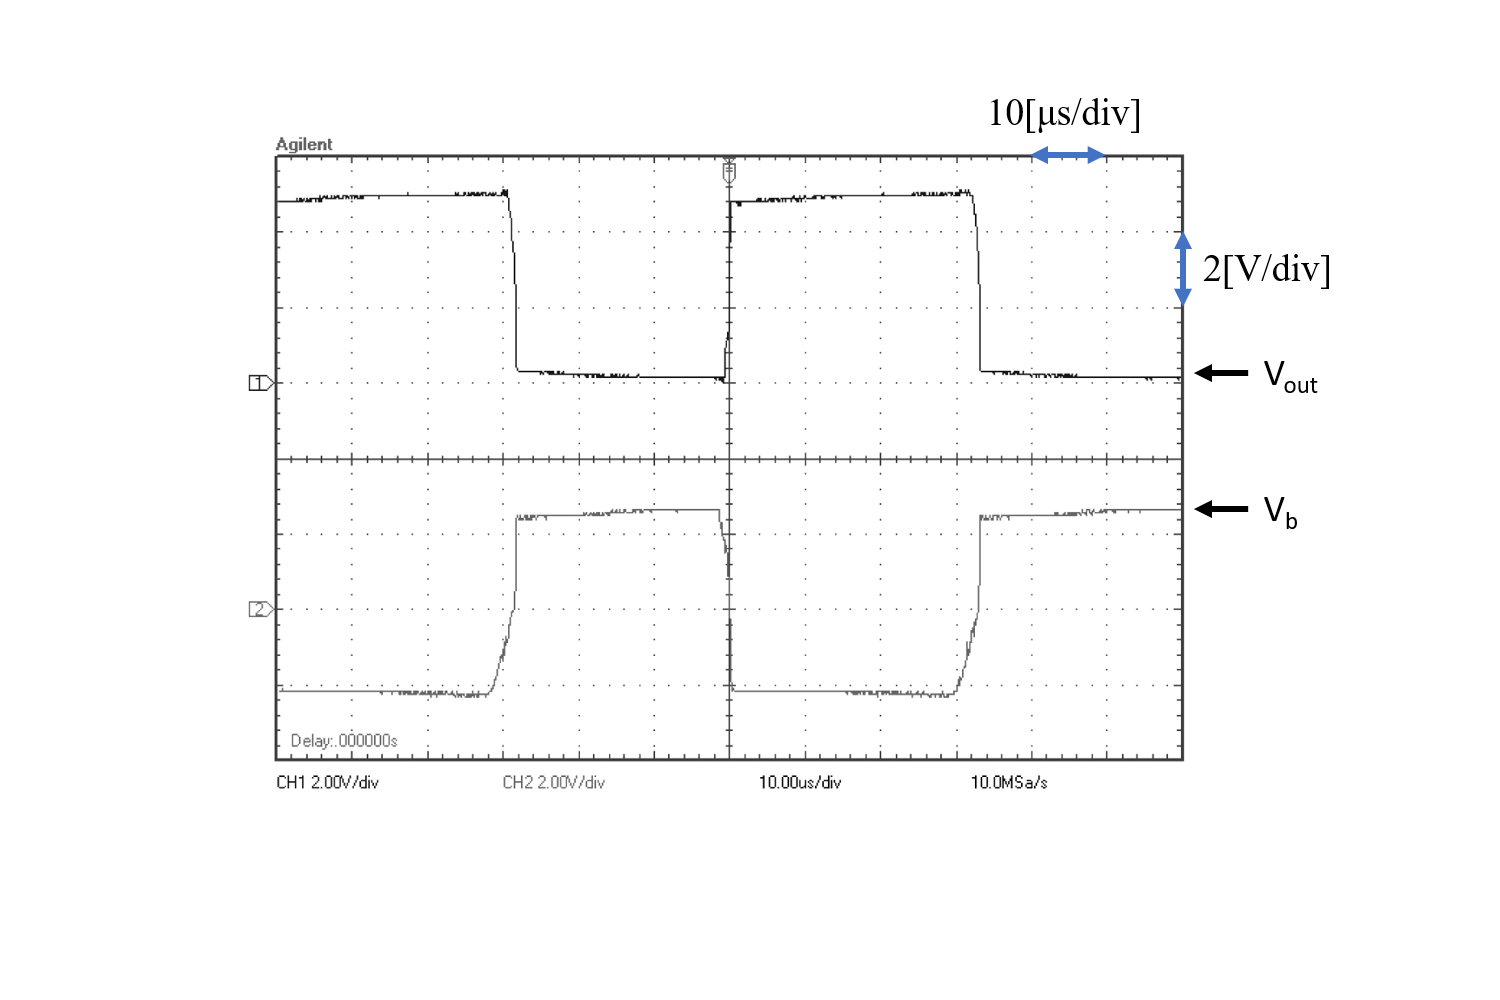
\includegraphics[width=\hsize]{images/223kc-Vout-Vb.png}
	\figcaption{Vout,Vbの出力波形}
	\label{223kc-Vout-Vb}
\end{figure}
\begin{figure}[H]
	\centering
	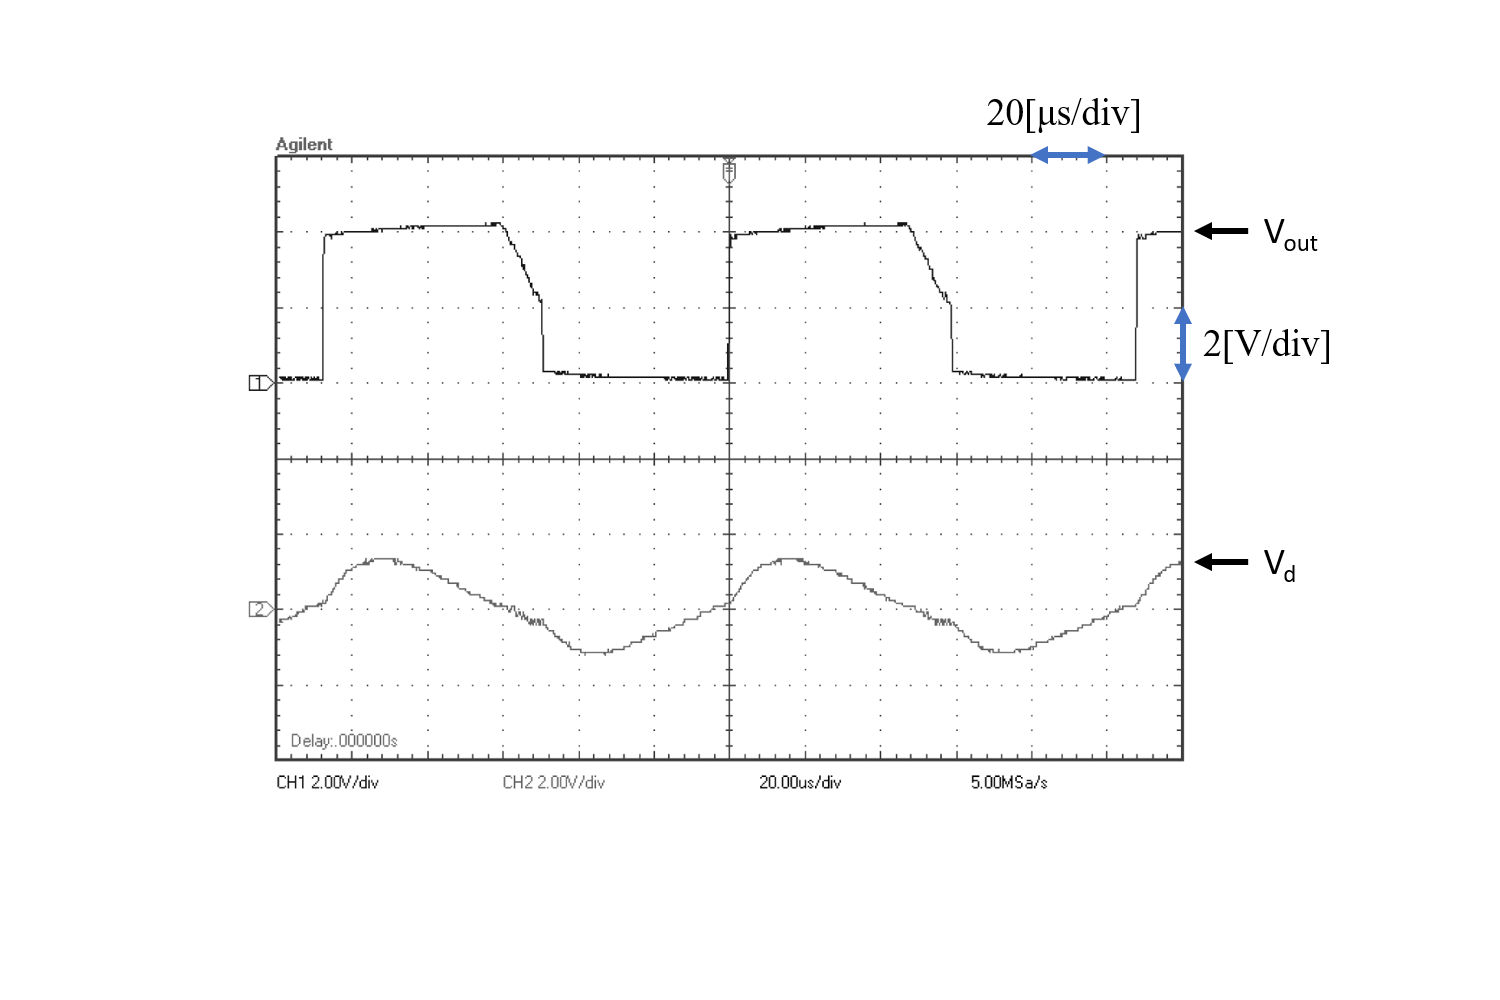
\includegraphics[width=\hsize]{images/223kc-Vout-Vd.png}
	\figcaption{Vout,Vdの出力波形}
	\label{223kc-Vout-Vd}
\end{figure}

\newpage
\section{考察}
\subsection{電源電流特性(貫通電流特性)の測定}
4.1の図\ref{fig:3.1}より,回路の電源電流は入力電圧2.1[V]~2.8[V]にかけて顕著に大きくなっていることが読み取れる.
使用したNANDICであるTC74HC00APのデータシートを確認すると,入力電圧が3.15[V]以上の時 H ,入力電圧が1.35[V]以下の時 L  として扱われることがわかる.
このとき,入力電圧がH,Lの閾値の間になると,内部回路に含まれるnMOS,pMOSの両方が同時にオンになってしまうタイミングが生まれる.
その結果,ICの内部で$V_{cc}$と$V_d$が短絡してしまい,大きい電流が流れていると考えられる.
この実験結果から,NANDICにHともLとも判別できない電圧を入力することは,電源電流を大きくしてしまい,回路の誤動作やICの破損を引き起こす可能性があるため,そのような入力は行うべきでないことがわかる.

また,データシートの動作範囲に入力上昇・下降時間という項目があり,回路中でTC74HC00APを使用する場合では入力の変化は$V_{cc}$=4.5[V]の場合500[ns]以下で使用するべきであることがわかる.

\subsection{入出力伝達特性の測定}
4.2の図\ref{fig:3.2}と4.1の図\ref{fig:3.1}を比較すると,図\ref{fig:3.2}で出力が変化している入力電圧の範囲は図\ref{fig:3.1}で電源電流が大きくなっている入力電圧の範囲と重なることがわかる.
また,データシートでは,特性として3.15[V]以上の時 H ,入力電圧が1.35[V]以下の時 L  として扱われるとあるが,実際にはそれより広い範囲で扱えるように見える.
しかし,前述の通りNANDICにHともLとも判別できない電圧を入力することは,電源電流を大きくしてしまい,回路の誤動作やICの破損を引き起こす可能性があるため,データシートの動作範囲内で使用するべきである.

\subsection{出力特性の測定}
4.3の図\ref{fig:3.3-0},図\ref{fig:3.3-1}を見ると,出力電圧に対して出力電流は比例しているが,その比例定数は非常に大きいことがわかる.

\subsection{非安定マルチバイブレータの特性}
4.4の図\ref{r105m-Vout-Va}~図\ref{223kc-Vout-Vd}から,コンデンサCの容量により周期Tは変化するが,波形はほぼ同じであることがわかる。
しかし,静電容量が大きい時,すなわち4.4.1,4.4.2の場合において,$V_d$の波形が乱れてい部分があった.
このいびつな波形が出力される頻度を調べるため,波形を取得する時間を長く設定し,同じオシロスコープを用いてデータを採取した.
以下,図\ref{r105m-ex},図\ref{224j-ex},図\ref{223kc-ex}にそのデータを示す.
\begin{figure}[H]
    \centering
    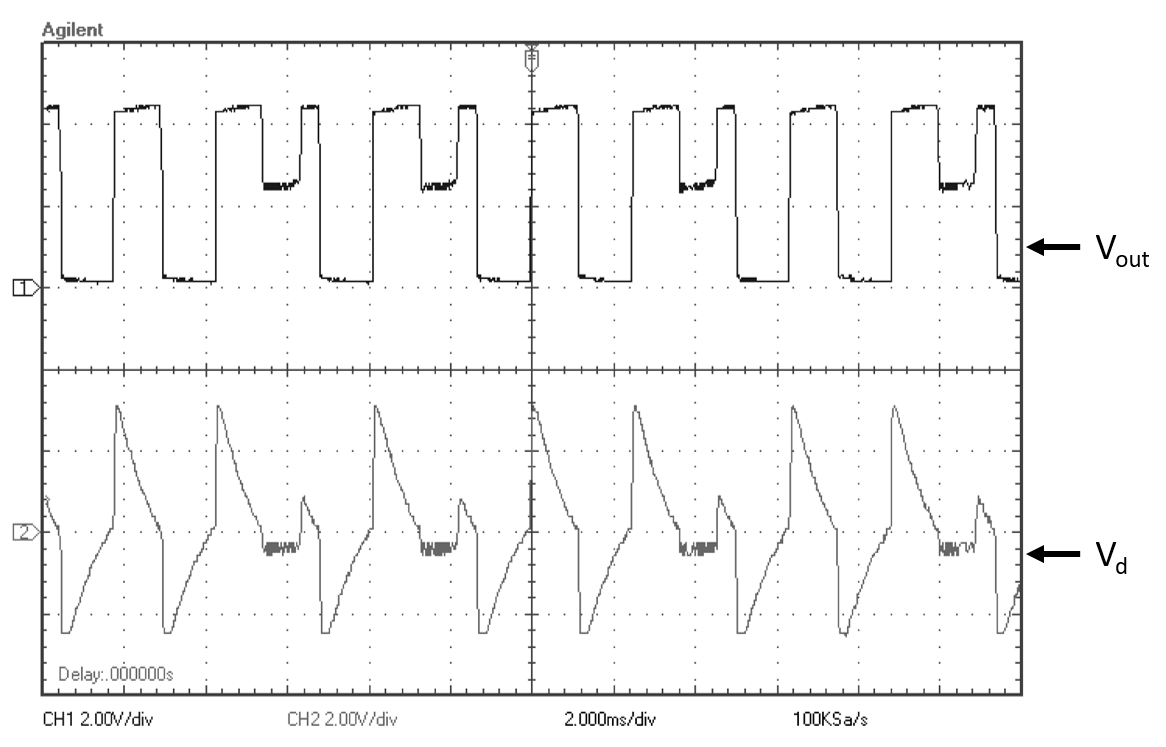
\includegraphics[width=\hsize]{images/r105m-ex.png}
    \caption{C = 1.000[$\mu$F]のときのVoutとVdの波形}
	\label{r105m-ex}
\end{figure}
\begin{figure}[H]
    \centering
    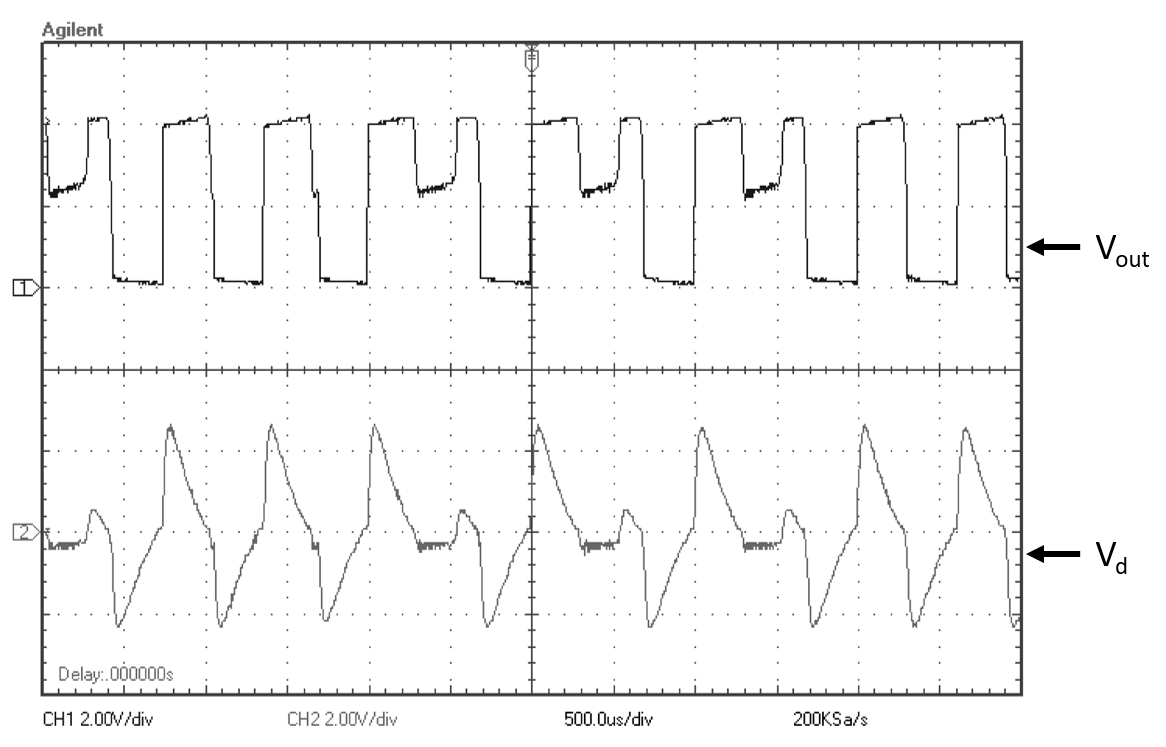
\includegraphics[width=\hsize]{images/224j-ex.png}
    \caption{C = 0.220[$\mu$F]のときのVoutとVdの波形}
	\label{224j-ex}
\end{figure}
\begin{figure}[H]
    \centering
    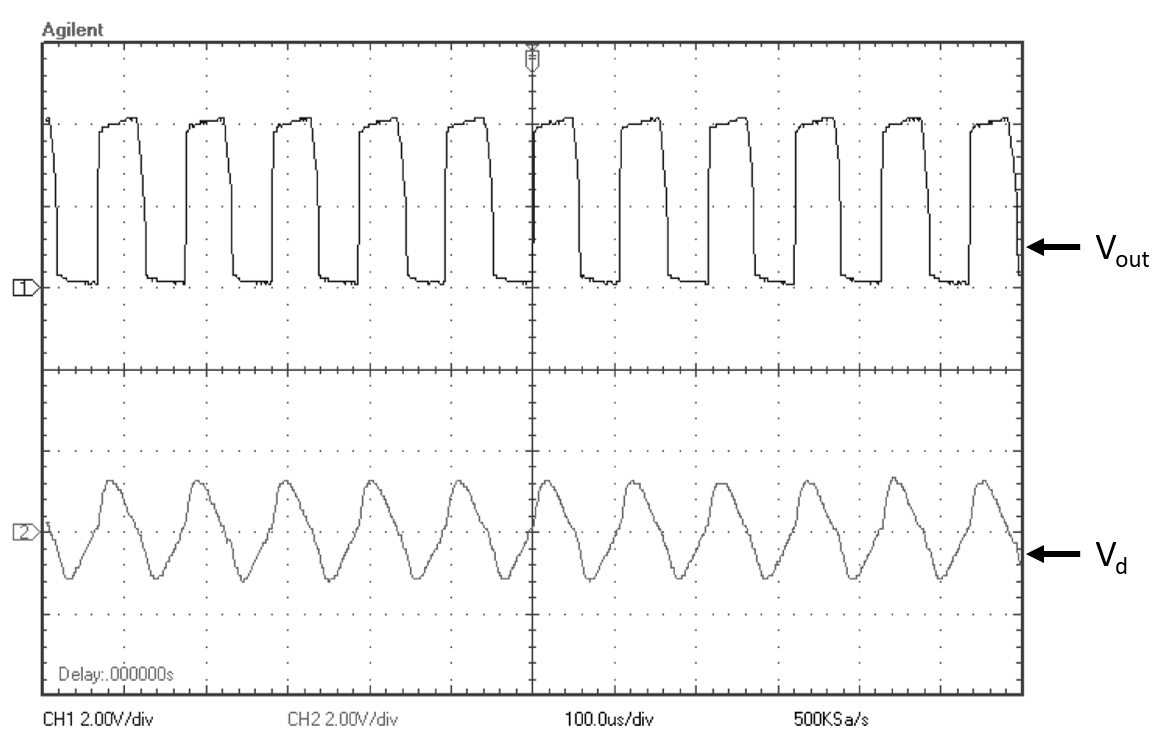
\includegraphics[width=\hsize]{images/223kc-ex.png}
    \caption{C = 0.022[$\mu$F]のときのVoutとVdの波形}
	\label{223kc-ex}
\end{figure}
これらの波形から,やはり4.4.1,4.4.2の条件下では波形の一部に乱れが生じていることがわかる.
これらの測定は静電容量Cのみを変化させた対照実験のため,この原因は静電容量の差にあると考えられる.
このとき,コンデンサは充放電を繰り返しているため,コンデンサの静電容量が大きいことにより,充放電に必要な時間が長くなってしまい,その間に変化した別の波形の作用によって電流の向き等が変化し,波形が乱れているのだと予想する.

\newpage
\subsection*{吟味事項}
\subsubsection{直流雑音余裕度とはなにか説明せよ.また,HCシリーズCMOSとTTLの直流雑音余裕度について説明し比較せよ.}
雑音余裕度(ノイズ・マージン)とは,ICの出力側と入力側のそれぞれにおいて,Hとして出力される(入力される),もしくはLとして入力される(出力される)電圧の差で表される.
これは,実際に回路を使用する際にどれくらいの大きさのノイズまで誤動作を起こさずに使用できるかという指標になる.
そのため,雑音余裕度が大きいものは安定性が良いといえる.

ここで,TC74HC00APと	SN74LS00Nを比較して,CMOSICとTTLICの雑音余裕度の差について議論する.\\
TC74HC00APでは,H側,L側それぞれの雑音余裕度は,$V_{cc}$を4.5[V]とすると,
\begin{equation}
	V_{OH} - V_{IH} = 4.4[V] - 3.15[V] = 1.25[V]
\end{equation}
\begin{equation}
	V_{IL} - V_{OL} =  1.35[V] - 0.1[V] = 1.25[V]
\end{equation}
	SN74LS00Nでは,H側,L側それぞれの雑音余裕度は,$V_{cc}$を4.5[V]とすると,
\begin{equation}
	V_{OH} - V_{IH} = 2.5[V] - 2.0V] = 0.5[V]
\end{equation}
\begin{equation}
	V_{IL} - V_{OL} =  0.8[V] - 0.4[V] = 0.4[V]
\end{equation}
となる.これらを比較すると,TTLの雑音余裕度はCMOSと比べて非常に小さく,CMOSを用いたほうが扱いやすいことがわかる.

\subsubsection{ファンアウトとはなにか,説明せよ.HCシリーズCMOSとTTLのファンアウトについて説明し,比較せよ.}
ファンアウトとは,一つの出力端子から駆動できる負荷ICの数のことである.
6.参考文献の5.に示すサイトを参考に,ファンアウトの計算方法をしめす.\\
CMOSでは,ファンアウトは$C_L / C_{IN}$で求められる.\\
TTLでは,入力・出力レベルがHの場合$I_{OH} / I_{IH}$,Lの場合$I_{OL} / I{IL}$を求め,このうち値の小さい方がファンアウト数となる.\\
これに従い計算を行うと,TC74HC00APでは, 
\begin{equation}
	C_L / C_{IN} = 50[pF] / 10[pF] = 5
\end{equation}
SN74LS00Nでは,
\begin{equation}
	I_{OH} / I_{IH} = 0.4[mA] / 20 [\mu A] = 20
\end{equation}
\begin{equation}
	I_{OL} / I{IL} = 8[mA] / 0.4[mA] = 20
\end{equation}
このとき,入力・出力レベルの違いによってファンアウト数が変わらないので,ファンアウト数は20.\\
以上より,TTLのファンアウト数はCMOSのそれを上回っており,負荷を多く接続する場合にはTTLを用いたICを使うほうが良いと考えられる.

\subsubsection{理論値の変化する所で電源電流が最大になるが,入力電圧$V_i$と電源電流$I_{cc}$との関係を調べ,この事実を定量的に説明せよ.}
5.1に記述したとおりである.

\subsubsection{非安定マルチバイブレータについて,各部波形を用いて動作原理を説明せよ.}
非安定マルチバイブレータの動作原理を,以下図\ref{マルチバイブレータ}に動作を表す図を示し,それに基づいて順を追って記述すると,
\begin{figure}[H]
	\centering
	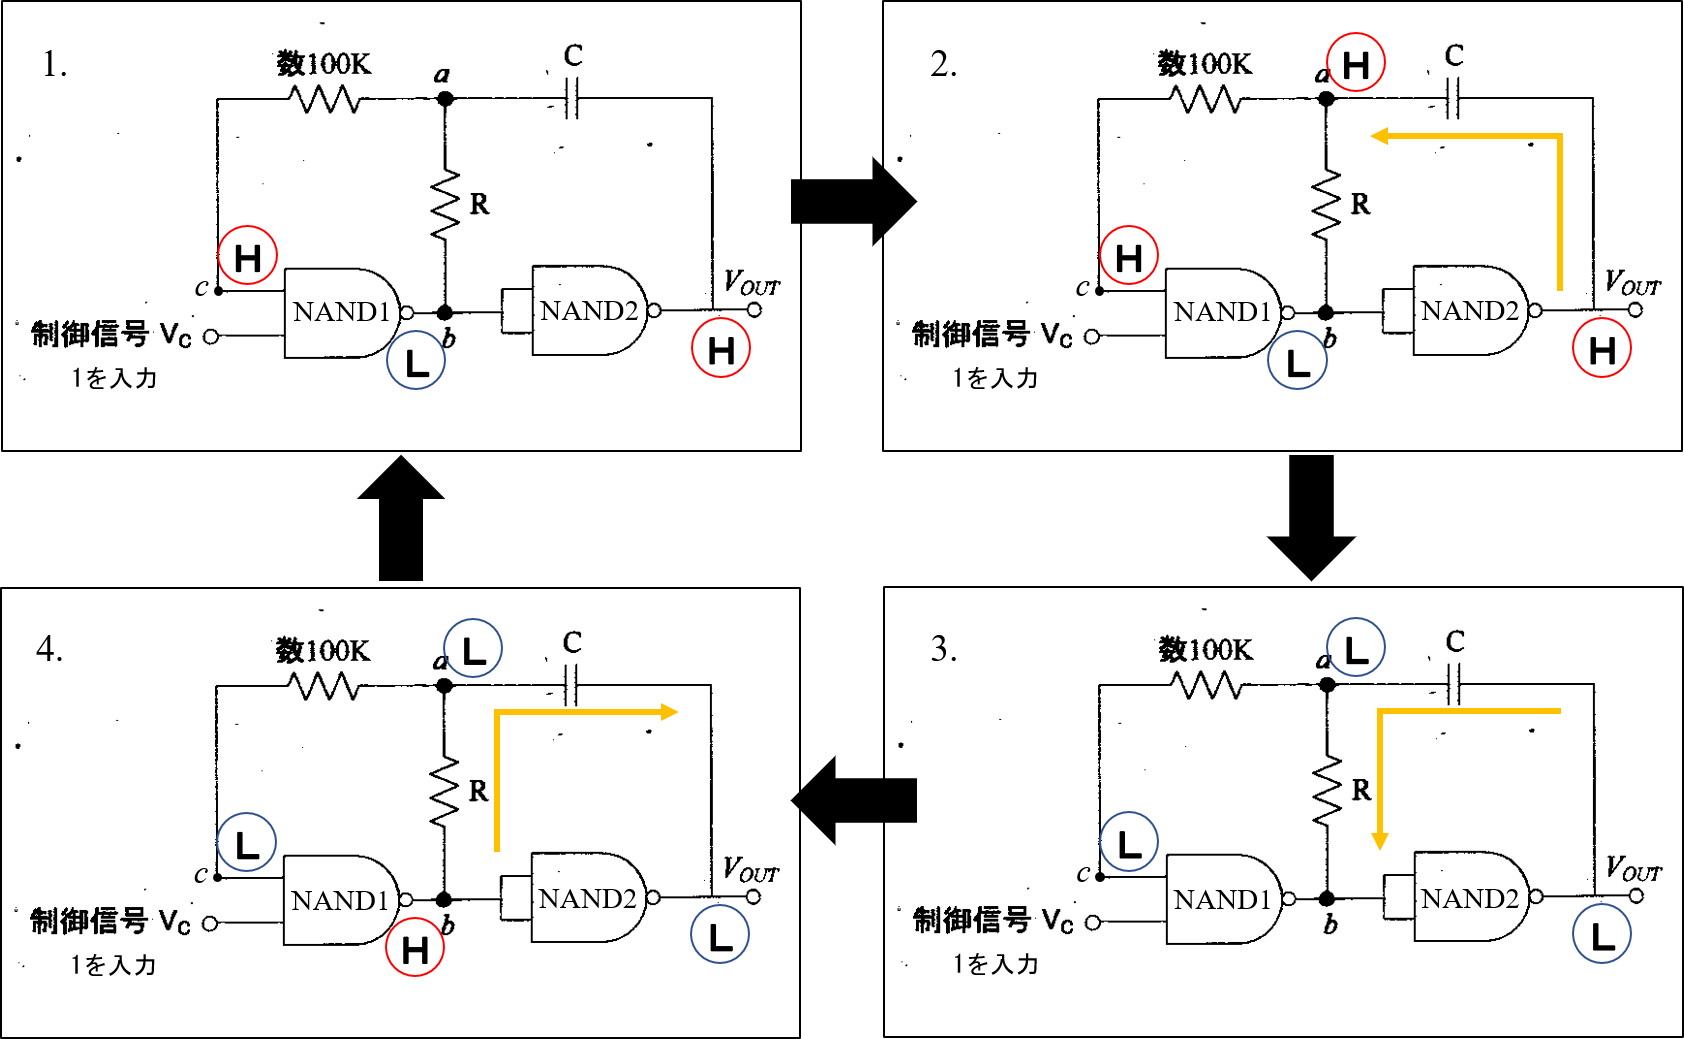
\includegraphics[width=\hsize]{images/動作原理.png}
	\figcaption{非安定マルチバイブレータの動作原理}
	\label{マルチバイブレータ}
\end{figure}
\begin{enumerate}
	\item 制御信号$V_C$を1にした瞬間 : コンデンサCが未充電で,かつNAND2の出力Voutを“H”とすれば,NAND1出力(b点)とNAND2入力が“L”,NAND1入力(c点)が“H”となる.
	\item 電圧の高いVoutから(a点),(b点)の経路で電流が発生し,コンデンサCの充電が開始される.このとき,(a点)と(b点)の間に抵抗Rに流れる電流とRの抵抗値に等しい電位差(電圧)が発生する.しかし,(a点)と(c点)は現時点では“H”なのでNAND1とNAND2の状態は保持される.
	\item コンデンサCの充電が進むと抵抗Rに流れる電流が小さくなるので,(a点)と(c点)の電圧が下がってくる.この値が“L”になると(b点)が“L”から“H”に反転してVoutが“H”から“L”になる.
	\item その瞬間に(b点)から(a点),Voutの経路で電流が流れ,コンデンサCの放電が始まる.放電が進むに従って(a点),(c点)の電圧が上昇し,この値が”H”の状態になると1の状態に戻り,結果としてNAND2の出力Voutから“H”,“L”を繰り返し出力する.
\end{enumerate}
また,波形については4.4に示したとおりである.

\subsubsection{非安定マルチバイブレータの周期を数種類(桁の異なる3種類)の容量Cについて測定し,理論値$T \approx 2CR\ln\{(V_H+V_S)/V_S\}$と比較検討してみよ.\\*	吟味事項4.及び比較結果より理論式が間違っていることが明らかであれば,新しい理論式を求めなさい.}
非安定マルチバイブレータの周期の理論値と測定値は表\ref{{tbl:3.4-C}}に示したとおりである.
これらの値を比較すると,多少誤差が見られる.
これは,周期の測定値はデジタルオシロスコープの測定結果から読み取ったことが原因の一つとして考えられる.

\section{感想}
今回の実験を通して,ICの基本的な使い方や特性等を知り,その測定法を学ぶことができた.\\
これまで趣味で行っていた電子工作では,まだまだ知識が足りなかったため,ICにパスコンをつないだことなどなかったので,今後の私生活にとっても非常に有益な実験であった.
しかし,実験データのとり方(特にディジタルオシロスコープのデータ)には問題があったので,あとで報告書を作成することを考えて,予め複数パターンのデータを取る.
また,必要になるかもしれない実験の過程等は写真等におさめておこうと思う.

ところで,今回から私は報告書を\LaTeX2eを用いて作成し,グラフについてはpython(matplotlib)を用いて作成している.
特に,\LaTeX2eの利点はマークアップ言語を記述するような間隔でレポートを作成できることであると思う.
これにより,文書の構造を明示的に扱うことができ,非常に心地良く報告書を作成できた.
また,グラフについてはpythonとそのライブラリであるmatplotlibを用いて作成したが,こちらは,使用するパソコンの性能によって処理にかかる時間に差があったり,グラフの書式の設定が面倒だったのでExcelで作成したほうが楽だったかもしれないと今頃になって後悔している.
一部図を作成する際にPowerPointを使用したときは,その相変わらずの有用さに心を打たれた.
閑話休題.

前述の通り,この実験は私にとって非常に面白く,また有益な実験であった.次回以降の実験も楽しみである.

\section{参考文献}
\begin{enumerate}
	\item 「宮崎技術研究所」の技術講座「電気と電子のお話」5.2.(2-B)\\ (URL : http://www.miyazaki-gijutsu.com/series4/densi0523.html)

	\item 1入力ゲートと入出力特性 - TTL | mixiコミュニティ\\ (URL : https://mixi.jp/view\_bbs.pl?comm\_id=478269\&id=9482402)

	\item TC74HC00AP データシート\\ (URL : https://toshiba.semicon-storage.com/info/docget.jsp?did=6907\&prodName=TC74HC00AP)

	\item SN74LS00N データシート\\ (URL : http://www.ti.com/lit/ds/symlink/sn7400.pdf)

	\item ファンアウト (URL : http://www.f-kmr.com/fanout.htm)
	
\end{enumerate}

\end{document}